% !TEX root = approx8.tex

\section{Corollaries of approximability and weighted
  complexity}\label{sec:complex}
The aim of this section is to prove Corollaries \ref{cor:no-t-b},
\ref{cor:quasi-rig}, and \ref{cor:link}, and to discuss some notions
of complexity that are then used to deduce Corollary
\ref{cor:no-t-b}. This type of complexity has interest in itself and
we start the section with a discussion of this topic, that is purely
algebraic in nature, in \S\ref{subsec:complex_alg}.  We continue with
the proof of Corollary \ref{cor:no-t-b} in \S\ref{subsec:non-v_Cor}.
In \S\ref{subsec:qrig-cor} and \S\ref{subsec:Gw-cor}, respectively, we
prove the other two corollaries.



\subsection{Complexity in TPCs}\label{subsec:complex_alg}

Most of this subsection is purely algebraic and can be read
independently of any considerations related to symplectic topology,
Fukaya categories and so forth.  In \S\ref{subsec:wconel} we introduce
the notions of complexity we are interested in, the most important one
being that of {\em weighted cone-length}. We also state the main
result of the subsection, Proposition \ref{prop:lower-bd}, providing a
lower bound for weighted cone-length in terms of a count of bars in a
certain barcode.  The proof of this proposition occupies the rest of
the subsection. In \S\ref{subsec:retr} we establish some algebraic
properties that lead to the inequality in Corollary
\ref{cor:nice-ineq} that reduces the statement of the proposition to
some properties of weighted cone-length in the homotopy category of
filtered chain complexes. These properties are established in
\S\ref{subsec:pers}.  In \S\ref{subsec:proof_Prop} the various
arguments are put together to show Proposition \ref{prop:lower-bd}. In
\S\ref{subsec:entrop} we introduce a notion of weighted categorical
entropy which is a weighted analogue of a similar notion introduced by
Dimitrov-Haiden-Katzarkov-Kontsevich \cite{DHKK:dyn_cat} and, as a
corollary of Proposition \ref{prop:lower-bd}, we estimate this
weighted entropy from below by the barcode entropy as defined by
\c{C}ineli-Ginzburg-Gurel \cite{CGG_bar_ent}. Finally, in
\S\ref{subsubsec:complex_Lag} we return to Lagrangians in cotangent
bundles and make some first comments concerning their complexity.

\

The setting of the subsection is that of a triangulated persistence category $\C$ endowed with the interleaving pseudo-metric 
$\dint$ as in equation (\ref{eq:d-int}). 
%We will make use of a simplified notion of TPC-approximability that reformulates point ii
%of Definition \ref{def:TPC-approx}. 
%
%
%\begin{dfn} \label{def:simple_approx}
%For some $\epsilon >0$, we say that $Y\subset \Ob(\C)$ is $\epsilon$-{\em approximable in} $\C$ if there exists a {finite} family
%$\F_{\epsilon}\subset \Ob(\C)$, called an $\epsilon$-{\em approximating family} for $Y$ in $\C$, such that 
%$$\dint(\ x, \Ob (\langle \F_{\epsilon}\rangle^{\Delta})\ ) < \epsilon, \forall x \in Y~.~$$
%The set $Y$ is called approximable in $\C$ if it is $\epsilon$-approximable for each $\epsilon >0$.
%\end{dfn} 
%
%It is easy to also formulate a corresponding retract version of approximability  by using $\dret$ from (\ref{eq:d-rint}) in Definition \ref{def:simple_approx} instead of $\dint$. 
%
%\begin{rem}\label{rem:relation-TPCapp}
%a.  Both $\dint$ and $\dret$ have shift-invariant versions where $\dint$, $\dret$ are, respectively, replaced by $\sdint$, $\sdret$. However, notice that the set 
%$\Ob (\langle \mathcal{S}\rangle ^{\Delta})$ where $\langle \mathcal{S} \rangle ^{\Delta}$ is the smallest
%sub-TPC of $\C$ containing $\mathcal{S}\subset \Ob (\C)$ is shift and translation invariant. It follows immediately that 
%$\dint(x, \Ob (\langle \F_{\epsilon}\rangle^{\Delta})) =\sdint(x, \Ob (\langle \mathcal{F}_{\epsilon}\rangle^{\Delta}))$ for all $x\in Y$, and similarly for $\dret$. 
%Thus, the regular and shift invariant versions of approximability in the sense of Definition \ref{def:simple_approx} 
%coincide and the same is true for retract approximability.
%
%
%b. Given a metric space $(X,d)$ and a quasi-isometric embedding $\Phi_{\eta}$  as at the point {\em i.} in Definition \ref{def:TPC-approx},  we see that point {\em ii.} in that definition is equivalent to $\Phi_{\eta}(X)\subset \Ob (\mathscr{Y}_{\eta})$ being $\epsilon$-approximable in $\mathscr{Y}_{\eta}$ in the sense of Definition \ref{def:simple_approx}. 
%\end{rem}

\subsubsection{Weighted generating rank and
  cone-length} \label{subsec:wconel} In the setting above consider
$X\subset \Ob(\C)$ and define the $\epsilon$-{\em generating rank}
of $X$ by:
\begin{equation}\label{eq:no-of-gen}
  g_{\C}(X; \epsilon) =
  \inf \bigl\{  \# (\F_{\epsilon})\
  |\  \F_{\epsilon}\subset \Ob (\C)   ,
  \   \forall x\in X, \
  d_{int}\bigl(x, \Ob(\langle\F_{\epsilon}\rangle ^{\Delta})\bigr)
  \leq \epsilon \bigr\}.
\end{equation} 
Here $\# (\mathcal{S})$ indicates the cardinality of the set
$\mathcal{S}$, and $\langle \mathcal{S} \rangle ^{\Delta}$ is defined
in~\S\ref{sb:tpc}.

Finiteness of the $\epsilon$-generating rank of
$X\subset \Ob(\C)$ is equivalent to $\epsilon$-approximability of
$X$ in $\C$, as seen by inspecting Definition \ref{def:simple_approx}.

\

A more important complexity measurement, also related to
approximability, is a weighted version of the classical notion of
cone-length of a topological space in homotopy theory \cite{Gan:cat},
\cite{Cor:cone-LS}, \cite{Cor:cone-SCat}.  We fix some preliminary
notation. Let $\C'$ be a triangulated category and let
$\F\subset \Ob(\C')$.  Consider a sequence
$\eta=(\Delta_{0},\ldots, \Delta_{m})$ of exact triangles in
$\C'$ of the form:
\begin{equation}\label{eq:triang-dec}\Delta_{i} \ \ : \ \ \
  F_{i}\longrightarrow A_{i}\longrightarrow A_{i+1}\longrightarrow
  TF_{i} \ \ , \ 0\leq i \leq m
\end{equation}
with $F_{i}\in \F$ and with $A_{m+1}=A$. We symbolically denote such a
sequence by $$\eta: A_{0} \stackrel{\F}{\rightsquigarrow} A$$ and we
let $\#(\eta)=m+1$ be the number of triangles in the sequence.  We
call the ordered family $(F_{0},\ldots, F_{m})$ the linearization of
$\eta$ and denote it by $\ell(\eta)$. By analogy with classical
topology, we will refer to each exact triangle as in
(\ref{eq:triang-dec}) as a {\em cone attachment over} $F_{i}$.  Assume
now that $\C$ is a TPC. In this case we will use the
notation $$\eta:A_{0}\stackrel{\F^{\Sigma, T}}{\rightsquigarrow} A$$
to refer to a sequence similar to (\ref{eq:triang-dec}) where
each triangle $\Delta_{i}$ is now {\em strict exact in}
$\C$. More specifically this means that each triangle
  $\Delta_i$ is now replaced by a strict exact triangle (in the sense
  of~\cite[Definition~2.42]{BCZ:tpc})
\begin{equation*} \label{eq:triang-dec-weighted} \Delta'_{i} \ \ : \ \
  \ F_{i}\longrightarrow A_{i}\longrightarrow A_{i+1}\longrightarrow
  \Sigma^{-w_i} TF_{i},
\end{equation*}
for some weight $w_i \geq 0$, $i = 0, \ldots, m$.

We emphasize that in this case the $F_{i}$'s are taken to be elements
in the set
$\mathcal{\F}^{\Sigma, T}=\{ T^{i}\Sigma^{\alpha} F \ | \ F\in \F ,
i\in \Z, \alpha\in \R\}$. The weight $w(\eta)$ of the decomposition
$\eta$, is defined as the sum of the weights of each of the triangles
$\Delta'_i$ in $\eta$, $w(\eta) = w_0 + \cdots + w_m$ (see
\cite{BCZ:tpc} for the basics on TPCs). If $\eta$ is of weight $0$, as
it will be the case in most of what follows, then each of the strict
exact triangles in $\eta$ is an exact triangle in the usual
triangulated category $\C^{0}$.
 
\begin{dfn}\label{def:w-cl}
  Fix $\C$ a TPC, as above, a family $\F\subset \Ob(\C)$, and also
  $\epsilon\in [0,\infty)$.  For any two objects $A, B$ of $\C$ the
  {\em $\epsilon$-weight cone-length of $A$ relative to $B$ with
    linearization in $\mathcal{F}$} is given by:
  \begin{equation}\label{eq:Number}
    N_{\C}(A, B;\F, \epsilon):=\inf\left\{  \#(\eta)\ \  | \ \ \eta: B\stackrel{\F^{\Sigma, T}}{\rightsquigarrow} A',  \  \ w(\eta)=0, \ \ \dint (A, A')\leq \epsilon \right\}.
  \end{equation}
\end{dfn}
In case the category $\C$ is clear from the context we write instead
$N(A,B;\F,\epsilon)$. Moreover, we write $N(A;\F,\epsilon)$ when
$B=0$, $$N(A;\F,\epsilon) := N(A, 0;\F,\epsilon)~.~$$ In short,
$N(A,B;\F,\epsilon)$ tells us how many iterated exact triangles in
the (usual) triangulated category $\C^{0}$ are needed to get
$\epsilon$-close to $A$ in the interleaving pseudo-distance,
starting from $B$, by attaching cones over objects of the form
$T^{i}\Sigma^{\alpha}F$, $F\in \F$, $\alpha\in\R$, $i\in \Z$.
 
\
 
The relation between weighted cone-length and approximability is that
if $\F$ is finite and $N_{\C}(A;\F,\epsilon) < \infty$,
$\forall \ A\in\Ob(\C)$, then $\F$ is an $\epsilon$-approximating
family in the sense of Definition \ref{def:simple_approx}, and
$g_{\C}(X;\epsilon) \leq \# (\F)$.
 
\begin{rem}\label{rem:cone-l} a. The definition of
  $N(A,B;\F,\epsilon)$ above is, in some sense, the simplest
  possible as it does not require any TPC machinery. Indeed, $\eta$ in
  (\ref{eq:Number}) consists of exact triangles in the usual sense, in
  $\C^{0}$, and $\dint(-)$ is the interleaving pseudo-metric which is
  already defined in a persistence category, see
  (\ref{eq:d-int}). Another measurement, more natural from the TPC
  perspective, can be defined by
  $$N'(A, B;\F,\epsilon)=\inf\{\ \#(\eta)\ \ | \ \
  \eta:B\stackrel{\F^{\Sigma, T}}{\rightsquigarrow} A\ \ , \ \
  w(\eta)\leq \epsilon \}~.~$$ This does not bring any essential
  new information because basic TPC algebra - see proof of Lemma 2.87
  in \cite{BCZ:tpc} - implies:
  $$N(A;\F,2\epsilon)\leq N'(A;\F,\epsilon)\leq  N(A;\F,\frac{\epsilon}{4})~.~$$

  b. Weighted cone-length satisfies some simple splitting inequalities
  associated with refinement of decompositions. These have
  generally a simpler expression for $N'(-,-)$ rather than for
  $N(-,-)$. For instance, we have
 $$N'(A,A'';\F,\epsilon'+\epsilon'')
 \leq N'(A, A';\F,\epsilon')+N'(A', A'';\F,\epsilon'')$$ which
 leads to the definition of fragmentation metrics on $\Ob (\C)$ (see
 \cite{BCZ:tpc}).

 
 c. The definition of cone-length above is very flexible.  By changing
 the family of objects over which cones are attached one obtains
 several other variants that are also of interest. One such choice,
 leading to smaller values for the resulting cone-length, is to
 replace $\F^{\Sigma, T}$ by
 $$ \F^{\otimes}=\{ F\otimes V \ |
 \ F\in \F, \ \ \ V \ \mathrm{\ is\ a\ finite\ dimensional, \ graded,\
   filtered \ vector\ space} \}$$ with the convention that
 $F\otimes \k[a] = \Sigma^{v(a)}T^{|a|}F$ where $\k[a]$ is the
 $1$-dimensional vector space generated by $a$ with
 degree $|a|$ and filtration level $v(a)$. Notice that
 $\F^{\Sigma, T}\subset \F^{\otimes}$. The resulting notion of cone
 length is such that, at each stage, one may attach a cone over a
 finite sum of copies of shifts and translates of elements of $\F$.
 We will denote this notion of cone-length by
 $N(A, B;\F^{\otimes},\epsilon)$.

 
 d. The numbers $N(A,B;\F,\epsilon)$ are decreasing in
 $\epsilon$ and, by taking $\epsilon \to \infty$, we obtain at
 the limit variants of the same notions that are often more familiar
 from standard topology and homological algebra.
\end{rem}
 
%\subsubsection{Lower bounds for weighted cone-length}\label{subsec:lowbd}
Under certain constraints, there exists a useful lower bound for
$N_{\C}(L;\F,\epsilon)$ which is well defined whenever $\F$ is
finite.  The inspiration for much of the algebraic considerations
related to the next result is found in
Dimitrov-Haiden-Katzarkov-Kontsevich \cite{DHKK:dyn_cat}.

\begin{prop} \label{prop:lower-bd}Let $\C$ be a TPC which is the homological category of a pre-triangulated category
  of filtered $A_{\infty}$-modules over a strictly unital filtered
  $A_{\infty}$-category and such that $\hom_{\C}(X,Y)$ is of finite
  type for all $X,Y\in \Ob(\C)$. Assume that $\F\subset \Ob (\C)$ is
  finite and consists of Yoneda modules. Under these assumptions,
  there exists a constant $k(\F)$ depending on the family $\F$ (and on
  $\C$) such that for every $L\in \Ob (\C)$ we have:
  $$N(L;\F,\epsilon)\geq k(\F) \sum_{F\in \F}\#
  \left( \mathcal{B}^{2\epsilon}_{\hom_{\C}(F,L)}\right)$$ where
  $\mathcal{B}^{\delta}_{V}$ is the barcode consisting of the bars of
  length greater than $\delta$ in the persistence module $V$.
\end{prop}
Recall that a persistence module is of finite type if its barcode
contains finitely many bars. The units of a filtered
$A_{\infty}$-category are always assumed to be in filtration $0$ (see
\S\ref{gio:fyon-def} for our conventions).

The conditions on $\C$ in the statement are satisfied for some of the
TPCs of Fukaya type that are among the main examples of interest in
the paper as well as for the homotopy category
$H^0(\mathcal{F}\ch^{fg})$ of finitely generated filtered
chain complexes over the field $\k$ (our ground field). We denote by
$\hfch$ the corresponding category without the finite generation
condition. Both are TPCs as shown in \cite{BCZ:tpc}.

The proof of the proposition appears in \S\ref{subsec:proof_Prop} and
is based on the results in the next two subsections that have
some interest in themselves.

\subsubsection{Weighted retracts}\label{subsec:retr} We fix here a
triangulated persistence category $\C$ and we refer again to
\cite{BCZ:tpc} for the basic definitions and notation relevant to
TPCs.

\

Similarly to (\ref{eq:Number}) we define the $\epsilon$-weight {\em
  retract} cone-length of $A$ relative to $B$ by:
\begin{equation}\label{eq:Number2}
  N^{r}_{\C}(A, B;\mathcal{F}, \epsilon)=\inf\left\{  \#(\eta)\ \
    | \ \ \eta: B\stackrel{\mathcal{F}^{\Sigma,T}}{\rightsquigarrow} A',
    \  \ w(\eta)=0, \ \ \dret  (A, A') \leq \epsilon \right\}
 \end{equation}
 (we recall that $\dret$ is defined in (\ref{eq:d-rint})).  In what
 follows it is useful to use the following terminology: given two
 objects $A,\bar{A}$ in $\C$ we will say that $A$ is {\em an
   $\epsilon$-retract of} $\bar{A}$ if
 $\dret(A, \bar{A}) < \epsilon$.  It is obvious that
 $$N^{r}_{\C}(A, B;\mathcal{F}, \epsilon)
 \leq N_{\C}(A, B;\mathcal{F}, \epsilon)~.~$$ The point of the
 definition is that the retract cone-length is, in practice, easier to
 estimate as we will see below. As before, if $B=0$ we omit it from
 the notation and we skip $\C$ if it is clear from context. The proof
 of Proposition \ref{prop:lower-bd} will make use \pbred{of} some
 algebraic properties of $N^{r}( -; -, \epsilon)$ and, indeed, the
 argument shows a stronger inequality than the one in the statement of
 the Proposition, namely:
 
 \begin{equation}\label{eq:ineq-r-bar}
   N^{r}(L;\F,\epsilon)\geq k(\F) \sum_{F\in \F}\#
   \left( \mathcal{B}^{2\epsilon}_{\hom_{\C}(F,L)}\right)
\end{equation}

\begin{rem}
  a. There is yet another variant of weighted retract cone-length
  which is defined by:
  $$\tilde{N}^{r}(A, B;\mathcal{F}, \epsilon)=
  \inf\left\{ N'(\bar{A}, B;\mathcal{F}, \epsilon) \ | \ \dret
    (A,\bar{A})=0\right \}.$$ This variant is particularly relevant if
  $\C^{0}$ is split complete in which case the condition
  $$\dret (A,\bar{A})=0$$ means that $A$
  is isomorphic to a direct summand of $\bar{A}$.

  b. It is easy to see using Remark \ref{rem:cone-l} a. that:
  $$N^{r}(A, B;\mathcal{F}, 2\epsilon)\leq
  \tilde{N}^{r}(A, B;\mathcal{F}, \epsilon)~.~$$


  c. The definition in (\ref{eq:Number2}) and the point a.~of the
  remark, are reminiscent of the relation between the
  Lusternik-Schnirelmann (LS) category and cone-length in topology,
  Theorem 1.1 in \cite{Cor:cone-LS}: the LS category of a topological
  space $X$ is the smallest integer $n$ such that $X$ is a homotopy
  factor of an $n$-cone.

\end{rem}


For the triangulated persistence category $\C$ and
$\mathcal{F}\subset \Ob (\C)$, assume that $\mathcal{F}$ is finite.
Let $G_{\F}=\oplus_{F\in\F}F$.  We will identify the family
$\{G_{\F}\}$ with the single object $G_{\F}$. One useful property of
the weighted retract cone-length is: 
\begin{lem}\label{lem:comp-sw}
  With the notation above we have
  $$N^{r}(A, B;G_{\F}, \epsilon) \leq N^{r}(A, B;\mathcal{F},
  \epsilon) \leq N^{r}(A, B;G_{\F}, \epsilon) \cdot
  \#(\mathcal{F}).$$
\end{lem}


The proof of the lemma is a simple exercise in manipulation of exact
triangles in triangulated categories, in this case in $\C_{0}$.  The
interest of the statement is that the cone-decomposition giving
$N^{r}(A,B; G_{\F},\epsilon)$ is a sequence of exact triangles as
in (\ref{eq:triang-dec}) but such that each $F_{i}$ is replaced by a
possible shift and/or translate of the single object
$G_{\mathcal{F}}$. As a result, it makes sense to consider the
measurement $N_{\C}^{r}(A,B; G,\epsilon)$ for any three objects
$A,B,G$ in $\C$.

\

Both variants of weighted retract cone-length, $N^{r}$ as well as
$\tilde{N}^{r}$, satisfy the additive splitting inequality in Remark
\ref{rem:cone-l} b but also a different, multiplicative one which
requires some assumptions on $\C$. Without weights, this type of
inequality was first noticed and used by
Dimitrov-Haiden-Katzarkov-Kontsevich \cite{DHKK:dyn_cat}. The
  weighted version will be instrumental here in proving
Proposition~\ref{prop:lower-bd}.

\begin{lem}\label{lem:hard-ineq} Assume that $\C$ is the persistence
 homological category associated with a
  pre-triangulated, filtered $A_{\infty}$-category. For any
  $A,G,G'\in \Ob (\C)$ we have:
  $$ N^{r}_{\C}(A;G,\epsilon)\leq N^{r}_{\C}(A;G',\epsilon')
  N^{r}_{\C}(G'; G,\epsilon'')$$ whenever
  $\epsilon \geq \epsilon ' + N^{r}_{\C}(A;G',\epsilon')
  \epsilon''$.

  The same formula remains true for $\tilde{N}^{r}(-;-,-)$ under a
  different assumption on $\C$, namely that $\C^{0}$ is split
  complete.
\end{lem}

\begin{rem} a. The relation tying
  $\epsilon, \epsilon', \epsilon''$ in the lemma is
  complicated but in this paper we will only need to use the case when
  $\epsilon''=0$ and $\epsilon=\epsilon'$.

  b. The weighted cone length $N_{\C}(-;-,\epsilon)$ also satisfies
  a multiplicative inequality of the type in Lemma \ref{lem:hard-ineq}
  but the precise formula is more complicated to state and thus we
  skip it here as it is not necessary later in the paper.

  c. The main examples of interest in this paper of categories $\C$ as
  in the first part of the Lemma are the homological category
  of filtered modules over a filtered $A_{\infty}$-category as well
  as, the simplest example, the homotopy category of filtered chain
  complexes.
\end{rem}

\begin{proof}[Proof of Lemma \ref{lem:hard-ineq}] The statement for
  $N^{r}_{\C}(-)$ is an immediate consequence of Lemma 6.12 in
  \cite{Bi-Co-Sh:LagrSh}.  We recall the statement of this lemma
  reformulated for filtered modules. Assume that $\mathcal{M}$ is an
  iterated cone of filtered $A_{\infty}$-modules (over $0$-shift
  maps):
  \begin{eqnarray*}
    \mathcal{M}=\tcn(\K_{s} \to \tcn(\K_{s-1}\to \ldots
    \to\tcn(\mathcal{N}\to \tcn(\K_{i-1} \to \ldots \to \\ \to
    \tcn (\K_{2}\to \K_{1})\ldots ))~.~
  \end{eqnarray*}
  Lemma 6.12 from \cite{Bi-Co-Sh:LagrSh} states that if $\mathcal{N}$
  is an $r$-retract of another filtered module $\mathcal{N}'$, then
  $\mathcal{M}$ is an $r$-retract of a filtered module $\mathcal{M}'$
  which is an iterated cone of the same form as $\mathcal{M}$ but with
  $\mathcal{N}'$ replacing $\mathcal{N}$ in the decomposition above.
  The proof of this result is based on the fact that in a category
  such as those in the statement of \ref{lem:hard-ineq} a homotopy
  commutative square has the property that the map induced between the
  cones over the two horizontal maps in the square can be expressed
  explicitly by a formula involving the two vertical maps and the
  commuting homotopy.

  This result is applied in our context as follows. We start with a
  decomposition in $\C^{0}$
  $\eta: 0\stackrel{(G')^{\Sigma,T}}{\cobto} \bar{A}$ and we assume
  that $A$ is an $\epsilon'$-retract of $\bar{A}$. We also assume
  that there is a second decomposition, also in $\C^{0}$,
  $\eta':0\stackrel{G^{\Sigma,T}}{\cobto}\bar{G}'$ and we assume that
  $G'$ is an $\epsilon''$-retract of $\bar{G}'$. By applying the
  algebraic result mentioned above to each of the terms in the
  linearization $\ell(\eta)$ of $\eta$ we transform $\eta$ into a new
  decomposition
  $\bar{\eta}:0\stackrel{(\bar{G}')^{\Sigma,T}}{\cobto} \bar{A}'$,
  still in $\C^{0}$, such that $A$ is now an
  $(\epsilon' + \#\ell(\eta) \epsilon'')$-retract of $\bar{A'}$.
  Finally, by refining each term in the linearization of $\bar{\eta}$
  by using the decomposition $\eta'$ we obtain the final decomposition
  $\bar{\eta}':0\stackrel{G^{\Sigma}}{\cobto} \bar{A}'$ which shows
  the claim (see Proposition 2.55 in \cite{BCZ:tpc} for the precise
  description of the refinement process).

  The argument for $\tilde{N}^{r}(-;--)$, under the assumption that
  $\C^{0}$ is split-complete, is similar but simpler as it does not
  require Lemma 6.12 from \cite{Bi-Co-Sh:LagrSh}, and we leave it as
  an exercise.
\end{proof}

One more property of weighted retract cone-length is needed.
\begin{lem}\label{lem:coef-ch} Assume that $\C$ satisfies the
  hypotheses in the statement of Proposition \ref{prop:lower-bd}. Let
  any $A, B\in\Ob(\C)$ and assume that $X\in \Ob(\C)$ is a Yoneda
  module. For any $\epsilon\geq 0$ we have:
  $$N^{r}_{\C}(A;B,\epsilon) \geq
  N^{r}_{\hfch}(\hom_{\C}(X,A);\hom_{\C}(X,B), \epsilon)~.~$$
\end{lem}

\begin{proof} Denote by $\D$ the pre-triangulated
  $A_{\infty}$-category of modules such that $\C=H^0\D$. Given
  that the underlying $A_{\infty}$-category is strictly unital, and
  that $X$ is a Yoneda module, we see that the functor
  $\hom_{\D}(X, -)$ transforms exact triangles in $\D$ into exact
  triangles in $[H^0(\mathcal{F}\ch)]^0$. This follows from
  the identification $\mathcal{M}(X)\cong \hom_{\D}(X,\mathcal{M})$,
  for each module $\mathcal{M}$, that is part of the properties of the
  Yoneda embedding functor - see \S\ref{gio:fyon-def} for the
  persistence setting - and the explicit formula giving the cone of a
  module morphism $\phi:\mathcal{M}\to \mathcal{N}$, \S3e in
  \cite{Se:book-fukaya-categ}. By applying $\hom_{\D}(X,-)$ this
  formula reduces to the usual formula giving the cone of the induced
  chain morphism
  $\phi_{X}:\hom(X,\mathcal{M})\to\hom(X,\mathcal{N})$. All these
  constructions respect filtrations and all the cones are taken over
  shift $0$ morphisms. As a result, exact triangles in $\C^{0}$ are
  represented by cone-decompositions in $\D$, these are sent by
  $\hom_{\D}(X,-)$ to corresponding cone-decomposition in
  $\mathcal{F}\ch^0$ that, in turn, give exact triangles in
  $[\hfch]^{0}$. The inequality in the statement is an immediate
  consequence of this observation.
\end{proof}

\

We proceed under the assumptions in the statement of Proposition
\ref{prop:lower-bd} and we also assume, as there, that
$\mathcal{F}\subset \Ob (\C)$ is finite and consists of Yoneda
modules. In particular, we can consider $G_{\F}=\oplus_{F\in\F}F$. In
this case, Lemma \ref{lem:coef-ch} implies that:
\begin{equation} \label{eq:NrC-GF}
  N^{r}_{\C}(A; G_{\F},\epsilon)\geq
  N^{r}_{\hfch}(\hom_{\C}(G_{\F}, A);
  \hom_{\C}(G_{\F},G_{\F}),\epsilon).
\end{equation}

Before we go on we temporarily introduce some simplified
  notation that will be used from now on till the end
  of~\S\ref{subsec:proof_Prop}. Namely, we will use $\k$ to denote two
  different (albeit closely related) things. Recall that throughout
  the paper $\k$ stands for the ground field for our (unfiltered)
  categories and chain complexes, but we will also denote by the same
  $\k$ the filtered chain complex with a single generator in degree
  $0$ and of filtration level $0$. When we want to specify that
  generator, say $x$, we will denote this chain complex also by
  $\k \langle x \rangle$.

Getting back to our considerations and continuing
  from~\eqref{eq:NrC-GF} we deduce from Lemma \ref{lem:hard-ineq}
  that
\begin{eqnarray*}
  N^{r}_{\hfch}(\hom_{\C}(G_{\F}, A);
  \hom_{\C}(G_{\F},G_{\F}), \epsilon) \cdot
  N^{r}_{\hfch}(\hom_{\C}(G_{\F}, G_{\F});\k,0)\geq \\
  \geq 
  N^{r}_{\hfch}(\hom_{\C}(G_{\F}, A); \k,\epsilon)
\end{eqnarray*}
%\pbred{\pbst{Here $\k$ represents the filtered chain complex with a
  %  single generator in degree $0$ and of filtration $0$. }}
 Combining
this with Lemma~\ref{lem:comp-sw} we deduce the next inequality.

\begin{cor}\label{cor:nice-ineq} Under the assumptions of Proposition
  \ref{prop:lower-bd} and for
  $$k(\F):=1/ N^{r}_{\hfch}(\hom_{\C}(G_{\F}, G_{\F});\k,0)$$ we have
  for each object $A$ of $\C$ and all $\epsilon\geq 0$:
  $$ N^{r}_{\C}(A;\F,\epsilon) \geq  k(\F)
  N^{r}_{\hfch}(\hom_{\C}(G_{\F}, A); \k,\epsilon)~.~$$
\end{cor}

\subsubsection{Weighted cone-length for filtered chain
  complexes}\label{subsec:pers}
The aim of this subsection is to examine the various notions of
weighted cone-length that we introduced before in the very basic but
important example when the triangulated persistence category $\C$ is
the homotopy category of filtered, finite dimensional chain complexes,
$\hfch^{fg}$, over the base field $\k$.

%\pbred{\pbst{As before, we denote by $\k$ the filtered chain complex
   % with a single generator, which is in degree $0$ and of filtration
%    $0$.}}

\begin{ex}\label{ex:element} The following statements hold in the
  category $\hfch^{fg}$.

  a) Each object $V$ in $\hfch^{fg}$ can be written as a finite direct
  sum, unique up to permutation, of translations of elementary
  filtered chain complexes of two types
  $$E_{2}(a, b)=\k(a, b: da=0, db=a), \ \mathrm{and}\ \ E_{1}(c)=\k(c
  : dc=0).$$ For each of the generators $x$ of these chain complexes
  we denote by $v(x) \in \mathbb{R}$ its filtration level. For
  $E_2(a,b)$ we assume $v(b)\geq v(a)$ with degrees $|a|=0$,
  $|b|=1$. For $E_1(c)$ we assume $v(c)=0$ and $|c|=0$. Note
    that this notation differs form other conventions common in the
    literature. For example, in~\cite[Section~2.5.2]{BCZ:tpc}
    $E_2(a,b)$ denotes a chain complex with two generators as above
    but $a$, $b$ stand for the filtration levels of these two
    generators rather than for the generators themselves (and
    similarly for $E_1(c)$). In our notation the barcode of the
    persistence homology $H(E_2(a,b))$ is $[v(a), v(b))$ while
    in~\cite{BCZ:tpc} this barcode is $[a,b)$.

  b) The translation $T$ acts by shifting degrees in the obvious way:
  $|T^{k}x|=|x|+k$ and the shift functor changes the filtration levels
  by $v(\Sigma^{\alpha} x)=v(x)+\alpha$.

  c) Recall that $\k\langle x \rangle$ also stands for the
  $1$-dimensional filtered chain complex over $\k$ with one
    generator $x$, with $|x|=0$, $v(x)=0$. We then have:
  $$E_{2}(a,b)=\tcn (\ \Sigma^{v(b)}\k \langle b \rangle \ \to \
  \Sigma^{v(a)}\k\langle a \rangle\ )$$ where the cone is taken over
  the map $b\to a$. As for $E_1(c)$, we have:
  $$E_{1}(c)\cong \Sigma^{v(c)}\k\langle c \rangle ~.~$$
  As a result, for $\C=\hfch^{fg}$ and $X=\mathcal{O}b(\hfch^{fg})$ we
  have $g(X;0)=1$ (see (\ref{eq:no-of-gen})) with
  $\mathcal{F}_{0}=\k\langle x\rangle $. Thus $\hfch^{fg}$ is
  $0$-approximable with generating rank equal to $1$.
\end{ex}

The next result is also elementary but less immediate. We fix some
additional notation. For a persistence module $K$, we denote by
$\mathcal{B}_{K}$ its barcode, by $\mathcal{B}^{\delta}_{K}$ the
barcode consisting of only the bars of length $> \delta$ in $K$, and
by $K^{\infty}$ the $\infty$-limit of the persistence module $K$ (it
is a vector space of dimension equal to the number of semi-infinite
bars in $K$). 
%\pbred{\pbst{Moreover, we will denote from now on the
 %  chain complex $\k\langle x\rangle $ simply by $\k$ in case the
  %  labeling of the generator is irrelevant.}}
\begin{lem}\label{lem:noc-chains}
  Let $V$ be a filtered, finite dimensional chain complex.  Then:
  \begin{equation}\label{eq:identi} N(V,0;\k,\epsilon)=
    N^{r}(V,0;\k,\epsilon)= 2\#
    \left(\mathcal{B}^{2\epsilon}_{H(V)}\right) - \dim_{\k}
    (H(V)^{\infty}) ~.~
  \end{equation}
\end{lem}

\begin{proof}
  For a filtered chain complex $V$ in our class and $\delta\geq 0$,
  let $V_{\delta}$ be the chain complex obtained by writing $V$ as a
  direct sum of elementary terms, as at point a) in Example
  \ref{ex:element}, and eliminating from the sum all the terms
  $E_{2}(a,b)$ with $v(b)-v(a)\leq \delta$. Up to a filtered
    chain homotopy equivalence of $V$ there is an obvious inclusion
  of chain complexes $i_{V,\delta}: V_{\delta}\to V$ as well as a
  projection $j_{V,\delta}:V\to V_{\delta}$.  It is easy to see that:
\begin{itemize}
\item[i.] $V$ and $V_{2\delta}$ are $\delta$ interleaved. This happens
  because the map
  $\eta^{V}_{2\delta}:\Sigma^{\delta}V\to \Sigma_{-\delta}V$ is easily
  seen to be chain homotopic to the composition $i_{V}\circ j_{V}$
  (because $\eta^{E_{2}(a,b)}_{2\delta}$ is null-homotopic if
  $v(b)-v(a)\leq 2\delta$).
\item[ii.] The dimension of $V_{2\delta}$ is given by
  $2\# (\ \mathcal{B}^{2\delta}_{H(V)}\ ) - \dim_{\k} (H(V)^{\infty})$.
  This is because a pair of generators $a,b$ in a term of type
  $E_{2}(a,b)$ (in the direct sum writing of $V_{2\delta}$) are
  associated with a finite bar of the form $[v(a),v(b))$ and each
  generator of type $c$ in a term $E_{1}(c)$ corresponds to one
  semi-infinite bar, and survives to a generator in $H(V)^{\infty}$.
\item[iii.] There exists an obvious cone decomposition
  $\eta:0\stackrel{\langle \k\rangle^{\Sigma,T}}{\cobto} V_{2\delta}$
  with a number of cones equal to the dimension of $V_{2\delta}$.
\end{itemize}
As a result of these three points we conclude that
$N(V,0;\k,\epsilon)\leq 2\# \left(
  \mathcal{B}^{2\epsilon}_{H(V)}\right) - \dim_{\k} (H(V)^{\infty})$.

To conclude the proof of (\ref{eq:identi}) we need to show that, if
$V$ is an $\epsilon$-retract of $W$, then $W$ is at least a
$\dim_{\k}(V_{2\epsilon})$-cone for a decomposition
$\eta':0\cobto W$ with a linearization with terms of the form
$\Sigma^{\alpha}T^{i}\k$ (these are the elements of
$\langle\k\rangle^{\Sigma,T}$).

To show this we first notice that for any $W$ in our class of filtered
chain complexes we have that any cone decomposition $\eta:0\cobto W$
in $(\hfch^{fg})^{0}$ (this is the $0$-level category of the
TPC $\hfch^{fg}$) with linearization terms in
$\langle\k\rangle^{\Sigma,T}$ has at least $\dim_{\k}(W_{0})$ terms,
where $W_{0}$ is obtained from $W$ by omitting all terms
  $E_{2}(a,b)$ such that $v(a)=v(b)$. Indeed, any such decomposition
is the image of a decomposition $\bar{\eta}:0\cobto W'$ in the
underlying category of filtered chain complexes,
$\mathcal{F}{\bf Ch}$, and there is a filtered quasi-isomorphism (with
$0$-shift) $\phi:W\to W'$.  The number of cones in $\bar{\eta}$ is at
least $\dim_{\k}(W')$ for dimension reasons. On the other hand,
$\phi|_{W_{0}}$ is injective (this can be seen by noting that $\phi$
induces an identification $\mathcal{B}_{W}\cong \mathcal{B}_{W'}$ and
$\mathcal{B}_{W}=\mathcal{B}_{W_{0}}$).  Therefore, it remains to show
that if $V$ is an $\epsilon$-retract of $W$, then
$\dim_{\k}(W_{0})\geq \dim_{\k}(V_{2\epsilon})$. If $V$ is an
$\epsilon$-retract of $W$ it is immediate that it also is an
$\epsilon$-retract of $W_{0}$. It is a simple exercise to show that
in this case $V_{2\epsilon}$ injects into $W_{0}$, which concludes
the proof of the lemma.
\end{proof}

\begin{rem}\label{rem:another-ineq}
  An argument similar to the proof of Lemma \ref{lem:noc-chains}
  shows: 
    \begin{equation}\label{eq:identi2} N(0,V;\k,\epsilon)= 2\#
      \left(
      \mathcal{B}^{2\epsilon}_{H(V)}\right) - \dim_{\k} (H(V)^{\infty})~.~
  \end{equation}
 As a result of this identity and (\ref{eq:identi}), and of the
triangular inequality in Remark \ref{rem:cone-l} b) we obtain rough
upper bounds for $N(V,V'; \k,\epsilon)$,
$N^{r}(V,V';\k,\epsilon)$ in terms of the barcodes of
$H(V)$ and of $H(V')$.
\end{rem}


\subsubsection{Proof of Proposition \ref{prop:lower-bd}}
\label{subsec:proof_Prop}
Using the preparatory material from the last two sub-subsections 
we can finalize the proof of Proposition \ref{prop:lower-bd}.

We start with two other simple algebraic remarks concerning filtered
chain complexes. For this let $V$ be a finitely generated, filtered
chain complex.  First, for any $\delta\geq 0$, we obviously have
the inequality
  $$ \#\left( \mathcal{B}^{\delta}_{H(V)}\right)
  - \dim_{\k}(H(V)^{\infty})\geq 0$$ which we rewrite as
$2 \ \#(\mathcal{B}^{\delta}_{H(V)})
  -\dim_{\k}(H(V)^{\infty})\geq \#(\mathcal{B}^{\delta}_{H(V)})$.
Secondly, if $V'$ is another chain complex in our class we have

  $$\# \left( \mathcal{B}^{\delta}_{H(V\oplus V')} \right)=\#
  \left(\mathcal{B}^{\delta}_{H(V)}\right) +\# \left(
    \mathcal{B}^{\delta}_{H(V')}\right )~.~$$  Combining these
relations with Corollary \ref{cor:nice-ineq} and Lemma
\ref{lem:noc-chains} and recalling $G_{\F}=\oplus_{F\in\F}F$ we
deduce: 
\begin{eqnarray*}
  N_{\C}(L;\F,\epsilon) \geq  N^{r}_{\C}(L;\F,\epsilon)
  \geq k(\F) N^{r}_{\hfch}(\hom_{\C}(G_{\F}, L); \k,\epsilon) \geq \\ \geq 
  k(\F)\cdot  \#
  \left( \mathcal{B}^{2\epsilon}_{\hom_{\C}(G_{\F},L)}
  \right)=k(\F)\sum_{F\in\F} \#
  \left(\mathcal{B}^{2\epsilon}_{\hom_{\mathcal{C}}(F,L)}\right)
\end{eqnarray*}

which shows the inequality (\ref{eq:ineq-r-bar}) and also
concludes the proof of the proposition. \qed
%\end{proof}

\subsubsection{Weighted categorical entropy.}\label{subsec:entrop} We introduce here a weighted notion of categorical entropy that is the weighted analogue of a notion introduced by Dimitrov-Haiden-Katzarkov-Kontsevich in \cite{DHKK:dyn_cat}. 

Consider a triangulated persistence category $\C$ and fix $X\subset \Ob (\C)$ as well as a family $\mathcal{F}\subset \mathcal{O}b(\C)$, as in \S\ref{subsec:wconel}.   

\begin{dfn}\label{def:entropy} Given a (set theoretic) map $\Psi:  X\to X$ and one object $A\in X$, the $\epsilon$-weighted categorical entropy of $\Psi$ at $A$, relative to $\F\subset \C$, is defined by
$$h_{\F}(\Phi; A,\epsilon)=\limsup_{n\to \infty} \frac{\log(N_{\C}(\Psi^{n}A;\F,\epsilon))}{n}$$
\end{dfn}
Notice that this definition is only of interest when $\F$ is an $\epsilon$-approximating family for $X$ in $\C$ (as in Definition \ref{def:simple_approx}) which we will assume from now on, otherwise there is no way to ensure that $N_{\C}(\Psi^{n}A;\F, \epsilon)$ is finite. In other words, TPC approximability is needed for this definition to make sense.

\begin{rem}\label{rem:variants_ent}
a. Of course, a similar notion can be defined using $N_{\C}^{r}(-;--)$ leading to a variant denoted by $h_{\mathcal{F}}^{r}(\Psi; A,\epsilon)$.

b. The numbers $h_{\F}(\Psi;A,\epsilon)$, $h_{\mathcal{F}}^{r}(\Psi; A,\epsilon)$  are decreasing functions in $\epsilon$. It is useful to allow for $\epsilon=\infty$. In that case, the weight constraints disappear and we obtain purely (triangulated) categorical notions. In particular,  when $\F$ is finite, the categorical entropy introduced in \cite{DHKK:dyn_cat}  
is given by  $h_{G_{\F}}(\Psi;A,\infty)$ with $G_{\F}=\oplus_{F\in\F}F$. 

c. By contrast to the un-weighted case, the weighted entropy definition depends on the choice of the family $\F$. 

d. There are also notions of {\em slow} entropy that are defined by formulae of a similar type, in analogy with the standard corresponding dynamical systems definitions. 
\end{rem}

We will now see that Proposition \ref{prop:lower-bd} implies that weighted categorical entropy  admits as lower bound a version of the barcode entropy introduced in \cite{CGG_bar_ent}.

\

To make this relationship precise we define the notion of barcode entropy that we will use here in the setting
of the TPC, $\C$.  We have as before the map $\Psi:X\to X$ and we pick two objects $A \in X$, $B\in \Ob(\C)$. We now consider the 
$\epsilon$-barcode entropy of $\Psi$ at $A$, relative to $B$:
\begin{equation}\label{eq:bar-code_ent}
\hbar(\Psi; A, B;\epsilon)=\limsup_{n\to \infty}\frac{\log\left( \# (\mathcal{B}^{\epsilon}_{\hom_{\C}(B,\Psi^{n}A)})\right)}{n}
\end{equation} 


\begin{cor}\label{cor:entr_rel} Assume that the assumptions in Proposition \ref{prop:lower-bd} are satisfied. In particular,  $\mathcal{F}$ is finite and all $\hom_{\C}(-,-)$ are finite type persistence modules.
We have the inequalities:
$$
h_{\F}(\Psi; A,\epsilon)\geq h^{r}_{\F}(\Psi; A,\epsilon) \geq  h_{G_{\F}}^{r}(\Psi; A,\epsilon)\geq \hbar(\Psi; A, G_{\F};2\epsilon)
$$
where $G_{\F}=\oplus_{F\in\F} F$.
\end{cor}

This follows directly from Proposition \ref{prop:lower-bd}, see also (\ref{eq:ineq-r-bar}).


\subsubsection{Weighted complexity of Lagrangians} \label{subsubsec:complex_Lag}
We return here to the geometric context from \S\ref{subsec:back} and discuss some implications of the nearby approximability Theorem \ref{thm:nearby} from the point of view of the complexity measurements
introduced earlier in this section. 

We start with some definitions of complexity that are natural from the point of view of TPC-approximability - 
see Definition \ref{def:TPC-approx} as well as Remarks \ref{rem:def-TPC-approx} and \ref{rem:relation-TPCapp}. 

\begin{dfn} Assume $(X,d)$ is TPC-approximable and that, for a fixed $\epsilon >0$, the quasi-isometric embeddings $$\Phi = \{\Phi_{\eta}\} \ , \ \Phi_{\eta}: (X,d)\to (\Ob (\mathscr{Y}_{\eta}), \bar{d}_{\mathrm{int}}^{\ \eta})~.~$$
 that are part of the $\epsilon$-TPC approximating data are fixed. 
 \begin{itemize}
\item[i.] The $\epsilon$-generating rank of $(X,d)$ relative to $\Phi$ is defined by 
$$g_{\Phi}(X;\epsilon)= \limsup_{\eta\to 0}\   g_{\mathscr{Y}_{\eta}}(\Phi_{\eta}(X);\epsilon)  $$ See  (\ref{eq:no-of-gen}) for the definition of $g_{\mathscr{Y}_{\eta}}$.
\item[ii.] At this point  fix also a corresponding family $\mathcal{F}_{\epsilon,\eta}\subset \Ob (\mathscr{Y}_{\eta})$ as in Definition \ref{def:TPC-approx}.  For some $\epsilon'\geq \epsilon$, the $\epsilon'$-cone-length of an element $a\in X$ relative to the family $\F_{\epsilon}= \{\F_{\epsilon,\eta}\}_{0< \eta<\epsilon }$  is given by:
$$N_{\Phi}(a; \F_{\epsilon},\epsilon')= \limsup_{\eta\to 0} \  N_{\mathscr{Y}_{\eta}}(\Phi_{\eta}(a); \F_{\epsilon,\eta}, \epsilon') ~.~$$
\end{itemize}
\end{dfn}

Notice that for $\epsilon_{1}\geq \epsilon_{2}\geq \epsilon$ we have $ N_{\Phi}(a; \F_{\epsilon},\epsilon_{1})\leq N_{\Phi}(a; \F_{\epsilon},\epsilon_{2})$.
These notions have properties very similar to those of the corresponding measurements from \S\ref{subsec:wconel}. In particular, given a map $\Psi : X\to X$ and assuming that $(X,d)$ is TPC-approximable we define the $\epsilon'$-weighted categorical entropy of $\Psi$ at $a\in X$, relative
to the approximating data ($\Phi$, $\F_{\epsilon}=\{\F_{\epsilon,\eta}\})$, for $\epsilon'\geq \epsilon$ by

\begin{equation}\label{eq:cat_entropy2}
h_{\Phi,\F_{\epsilon}}(\Psi;a,\epsilon')=\limsup_{n\to\infty}\frac{\log  N_{\Phi}(\Psi^{n}a;\F_{\epsilon},\epsilon')}{n}~.~
\end{equation}

We also have similar measurements for the corresponding retract notions that will be denoted by  
$N^{r}_{\Phi}(a; \F_{\epsilon},\epsilon')$, $h^{r}_{\Phi,\F_{\epsilon}}(\Psi;a,\epsilon')$
respectively. 
\begin{rem}\label{rem:tb_complex} 
 Assume that the metric space $(X,d)$ is totally bounded and that it is TPC-approximable (respectively, retract-approximable) with a system
  of $(A,\eta)$-quasi-isometric embeddings $\Phi=\{\Phi_{\eta}\}$ and a corresponding family $\{\F_{\epsilon,\eta}\}$ as above. 
Then, for each fixed $\epsilon$, there exists $K >0$ depending on $(X,d)$, $\Phi$ and $\{\F_{\epsilon,\eta}\}$ 
such that $$N_{\Phi}(a;\F_{\epsilon},2\epsilon)\leq K$$ (respectively, $N^{r}_{\Phi}(a;\F_{\epsilon},2\epsilon)\leq K$) 
for all $a\in X$. This is a simple exercise: the bound $K$ is given by considering a finite $\epsilon_{1}$-net of $(X,d)$, $x_{1},\ldots, x_{k}\subset X$
such that $\epsilon_{1}/A < \epsilon$ and  taking $$K=\max_{i} N_{\mathscr{Y}_{\eta'}} (\Phi_{\eta'}(x_{i});\mathcal{F}_{\epsilon,\eta'}, \epsilon_{1}) \ \ (\mathrm{respectively}\ K=\max_{i} N^{r}_{\mathscr{Y}_{\eta'}} (\Phi_{\eta'}(x_{i});\mathcal{F}_{\epsilon,\eta'}, \epsilon) \ )$$  for some $\eta' < \epsilon$. In particular, if $(X,d)$ is totally bounded, 
for all $x\in X$ and any map $\Psi:X\to X$
the entropies $h_{\Phi,\F_{\epsilon}}(\Psi; a, 2\epsilon)$ and $h^{r}_{\Phi,\F_{\epsilon}}(\Psi; a, 2\epsilon)$ vanish. Thus, to show that $(X,d)$ is not totally bounded, it is enough to find one $\epsilon>0$ and a sequence $a_{k}\in X$ such that 
$N_{\phi}(a_{k};\F_{\epsilon}, 2\epsilon)\to \infty$ in $k$.
\end{rem}

We now turn to geometry.  We have shown in \S\ref{sec:nearby} that the metric space $$\mathcal{L}(N)=(\lag^{(ex)}(D^{\ast}N), d_{\gamma})$$ is approximable in the sense of Definition \ref{def:TPC-approx}. 
In \S\ref{subsubsec:local_approx_d} and \S\ref{subsubsec:amb_approx_d} we produced two types of TPC  $\epsilon$- approximating data for this space: $(\Phi, \F_{\epsilon})$ in the first case and $(\Phi', \F'_{\epsilon})$ in the second, which is only {\em retract} approximating. We referred to the first type as {\em local} and to the second as {\em ambient}.

\

To improve readability we recall the basic features of these two choices of approximating data.
The family $\Phi=\{\Phi_{\eta}\}$ of quasi-isometric embeddings 
consists of Yoneda embeddings - see \S\ref{subsec:nearby-TPC}:
$$\Phi_{\eta}= \mathcal{Y}_{\epsilon', p}: \lag^{(ex)}(D^{\ast}N)\to \Ob (\msc_{p})~.~$$ 
Here  $\msc_{p}$ are persistence homology categories of filtered $A_{\infty}$-modules over the filtered 
Fukaya category $\fuk(\lag^{(ex)}(D^{\ast}N), p)$ constructed for the choice of perturbations $p$, with $\nu(p) < \eta$ and $\epsilon'<\epsilon$. 
The family $\F_{\epsilon}$ consists of modules corresponding to a finite family 
$\{ F_{0},\ldots,  F_{x_{m}}\}$ of fibers of $D^{\ast}N$ where $\{ x_{0},x_{1},\ldots, x_{m}\}$ are the critical points of an auxiliary Morse function 
$\varphi_{N,K,\delta}:N\to [0, K]$.
The family $\Phi'$ is very similar except that the place of $\msc_{p}$ is taken  by the persistence derived category 
$$\mathscr{D}_{p}(E)=PD(\fuk(\mathcal{L}ag^{(ex)}(E), p))$$
that is constructed using the auxiliary Lefschetz fibration $\bar{h}:E\to \mathbb{C}$ (see \S\ref{subsec:Lef-Dehn})
 that itself depends on $\varphi_{N,K,\delta}$. The family $\F'_{\epsilon}$ consists of the Yoneda modules of 
Lagrangian spheres $\hat{S}_{x_{i}}$, one for each critical point of $\varphi_{N,K,\delta}$ and such that
$\hat{S}_{x_{i}}\cap D^{\ast}N=F_{x_{i}}$.

In essence, one can view the approximability results in $\msc_{p}$ as obtained by pull-back from those
in $\mathscr{D}_{p}(E)$. Notice though that $(\Phi',\F'_{\epsilon})$  is only  retract $\epsilon$-approximating,  as indicated in Corollary  \ref{thm:nearby_far}.

\begin{rem}\label{rem:coherence}
a. Recall that the comparison functors $\mathcal{H}_{p,q}:\msc_{p}\to \msc_{q}$ are TPC-functors for $p \preceq q$.  
They also preserve the generating families $\F_{\epsilon}$  in the sense that they send
the module  corresponding to a fibre $F_{x_{i}}$ in the $p$-category $\msc_{p}$ to a module $0$-isomorphic to the  module associated to the same $F_{x_{i}}$ in $\msc_{q}$.  As a result, with $\epsilon$ fixed, our approximating families
$\F_{\epsilon}$ are no longer dependent of $\eta$. Moreover, for each $L\in \lag^{(ex)}(D^{\ast}N)$
we have $$N_{\msc_{p}}(L;\F_{\epsilon}, \epsilon)\geq  N_{\msc_{q}}(L;\F_{\epsilon}, \epsilon)$$
as soon as $p\preceq q$. The same remark also applies to the system of categories $\{\mathscr{D}_{p}(E)\}_{p}$ and
the family $\F'_{\epsilon}$, and leads to the same inequality, with $\mathscr{D}_{-}(E)$ in the place of $\msc_{-}$ and as well with $N^{r}(-;-\epsilon)$ replacing $N(-;-\epsilon)$.

b. In the setting above we also have the inequality:
$$N_{\msc_{q}}(L;\F_{\epsilon}, \epsilon)\geq  N_{\msc_{p}}\left(L;\F_{\epsilon}, \epsilon + c |\eta(p)-\eta(q)|\right)$$ also under the assumption
$p\preceq q$ and for $c$ a constant independent of $L$. 
\end{rem}


\

Given that the number of elements in $\F_{\epsilon}$ and in $\F'_{\epsilon}$ is
equal to the number of critical points of $\varphi_{N,K,\delta}$  we deduce:
$$g_{\Phi}(\mathcal{L}(N);\epsilon)\leq  \# \ \Crit (\varphi_{N,K, \delta})$$
as well as the same inequality for $\Phi'$.
When $\epsilon \to 0$ the number of elements in $\F_{\epsilon}$ and $\F'_{\epsilon}$ 
goes to $\infty$ at a rate that can be estimated through the construction in  \S\ref{subsec:Morse}.

\

We now discuss in the same context and with the same notation the $\epsilon$-weight cone-length
$N_{\Phi}(L;\F_{\epsilon}, \epsilon)$ for $L\in \lag^{(ex)}(D^{\ast}N)$.  






  
An upper bound for this cone-length can be obtained by counting all the exact triangles $\Delta_{i,j}$ from (\ref{eq:tr-ref}) that  give the decomposition of $L$. As a result, $m(i)\leq 2 \#(\mathcal{B}_ {HF(\hat{S}_{x_{m-i}}, L_{i})})$ and 
 thus:
 \begin{equation}\label{eq:upperBars}N_{\Phi}(L;\F_{\epsilon},\epsilon)\leq\sum_{i=0}^{m}2 \#(\mathcal{B}_ {HF(\hat{S}_{x_{m-i}}, L_{i})}) ~.~
 \end{equation}
The Lagrangians $L_{i}\subset E$ are related through Dehn  twists  - as discussed in \S\ref{subsubsec:back_to_alg}: $L_{m+1}=L$,  $L_{m-i}=\tau_{\hat{S}_{i}}(L_{m-i+1})$.
As a result, we can obtain iteratively an upper bound for $\#(\mathcal{B}_{HF(\hat{S}_{x_{m-i}}, L_{i})})$, and, moreover it is easy to see that there exists a constant $k'(\F_{\epsilon})$, independent of $L$, as well as $\epsilon''>0$, $\epsilon'' \ll \epsilon$, depending again on $\F_{\epsilon}$ and not on $L$, such that
\begin{equation}\label{eq:upper_bound}
N_{\Phi}(L;\F_{\epsilon}, \epsilon)\leq k'(\F_{\epsilon})\ \max_{S\in \F_{\epsilon}}\ \left( \#(\mathcal{B}^{\epsilon''}_{HF(S,L)}) \right)
\end{equation}
These estimates are, of course, first established for $N_{\mathscr{Y}_{\eta}}(\Phi_{\eta}(a); \F_{\epsilon,\eta}, \epsilon)$ in  $\msc_{p}^{\epsilon}$ for $\nu(p)$ sufficiently small. By making $\nu(p)\to 0$ we see that they apply  also to $N_{\Phi}(L;\F_{\epsilon}, \epsilon)$, as stated above. 
The estimates  (\ref{eq:upperBars})  and (\ref{eq:upper_bound}) remain obviously true also for $\Phi',\F'_{\epsilon}$ by using $N^{r}_{\Phi'}( - )$ in that case.  

\

In the opposite direction, from Proposition \ref{prop:lower-bd}  together with the stronger form in (\ref{eq:ineq-r-bar}) we deduce a lower bound for weighted cone-length and entropy relative to the data $(\Phi',\F'_{\epsilon})$:

\begin{cor} \label{cor:ineq_bar2} For each $L\in \lag^{(ex)}(D^{\ast}N)$ and $\epsilon'\geq \epsilon$ we 
have:
$$N^{r}_{\Phi'}(L;\F'_{\epsilon},\epsilon')\geq k(\F'_{\epsilon}) \sum_{S\in \F'_{\epsilon}} \#(\mathcal{B}^{2\epsilon'}_{HF(S,L)})$$
for a constant $k(\F'_{\epsilon})$  only depending on the family $\F'_{\epsilon}$ and we also have:
$$h^{r}_{\Phi',\F'_{\epsilon}}(\Psi; L ,\epsilon')\geq  \hbar(\Psi; L, G_{\F'_{\epsilon}}; 2\epsilon')$$ 
for $G_{\F'_{\epsilon}}=\oplus_{S\in \F'_{\epsilon}} S$.
\end{cor}
Corollary \ref{cor:ineq_bar2} is stated for the ambient $\epsilon$-TPC -approximating data $(\Phi',\F'_{\epsilon})$. This is essential for two reasons: first, the category  $\mathscr{D}_{p}(E)$ has the property that $\hom_{\mathscr{D}_{p}(E)}(A,B)$ is a persistence module of finite type $\forall A, B\in \Ob (\mathscr{D}_{p}(E))$, as noted in Remark  \ref{rem:compare_data}, and, secondly, the family $\F'_{\epsilon}$ consists of Yoneda modules. Thus, we may apply 
Proposition \ref{prop:lower-bd} for each $\mathscr{D}_{p}(E)$ 
and by then letting $\nu(p)\to 0$ the statement follows. In contrast,  it is not clear whether a similar statement is valid
for the local approximating data $(\Phi, \F_{\epsilon})$. Indeed, even the constant $k(-)$, introduced in Corollary \ref{cor:nice-ineq}, is not {\em apriori} well-defined for $\F_{\epsilon}$. 

\begin{rem}\label{rem:entrop_bars}
In the setting above,  by combining  Corollary \ref{cor:ineq_bar2}
and (\ref{eq:upper_bound}) we deduce

\begin{equation}\label{eq:entropy2}\hbar(\Psi; L, G_{\F'_{\epsilon}}; \epsilon'') \geq h^{r}_{\Phi',\F'_{\epsilon}}(\Psi; L ,\epsilon) \geq 
\hbar(\Psi; L, G_{\F'_{\epsilon}}; 2\epsilon) \ \  \mathrm{for\ }\ 0<\epsilon'' \ll \epsilon
\end{equation}
which shows that, in this situation ($M=D^{\ast}N$ etc),  weighted categorical entropy is very closely related to the barcode entropy from \cite{CGG_bar_ent}.  In \cite{DHKK:dyn_cat} the authors obtain an upper bound for (the unweighted) categorical entropy by an algebraic approach that is  more general than the one used here so that, in principle, one expects an inequality such as (\ref{eq:entropy2}) to remain true in
wider generality.
\end{rem}

\subsection{Non-vanishing weighted categorical entropy and Corollary \ref{cor:no-t-b}}
\label{subsec:non-v_Cor} The aim of this subsection is to produce a class of examples with non-vanishing $\epsilon$-weighted categorical entropy in the sense of (\ref{eq:cat_entropy2}) but with vanishing  ``classical'' categorical entropy. We formulate this more precisely in the next statement. 

\begin{prop}\label{cor:hyp_ent} Let $(N,\mathtt{g})$  be a closed hyperbolic manifold. Consider the metric space 
$(\lag^{(ex)}(D^{\ast}N), d_{\gamma})$ and, for some small $\epsilon$, fix the ambient $\epsilon$-TPC - approximating data
$(\Phi',\F'_{\epsilon})$ as recalled in \S\ref{subsubsec:complex_Lag}.
There exists  a Lagrangian $L\in\lag^{(ex)}(D^{\ast}N)$ Hamiltonian isotopic to the zero section and a Hamiltonian diffeomorphism $\Psi: D^{\ast}N\to D^{\ast}N$ with support inside $D^{\ast}N$, such that
$$h^{r}_{\Phi',\F'_{\epsilon}}(\Psi; L, 2\epsilon)>h^{r}_{\Phi',\F'_{\epsilon}}(\Psi;L,\infty)=0$$
where the relevant $\epsilon$-weighted entropy is defined in (\ref{eq:cat_entropy2}).
\end{prop}

The result 
means that filtered categorical algebra is sensitive to the dynamics in a cotangent bundle in ways in which the non-filtered version is not.  Moreover, in view of Remark \ref{rem:tb_complex}, this proposition implies one part of Corollary \ref{cor:no-t-b} from the introduction, namely that the metric space $(\lag^{(ex)}(D^{\ast}N), d_{\gamma})$ is not totally bounded. The second part of the Corollary that refers to $M=S^{2}$ and with 
$\lag(S^{2})$ consisting of equators is addressed in \S\ref{subsec:tb_S2}.

\

The vanishing of the non-weighted categorical entropy, $h^{r}_{\Phi',\F'_{\epsilon}}(\Psi;L,\infty)$, in the statement is immediate  because  all $\Psi^{n}L$ are Hamiltonian isotopic to the zero section and thus, without weight constraints, they admit cone-decompositions with the same number of terms. 

\

Till now our arguments did not depend on the ground field $\k$, however from this point on we will
assume in this subsection that $\k=\Z_{2}$.

%Notice that any Hamiltonian diffeomorphism  $\Psi$ with support inside $D^{\ast}N$ trivially extends to $E$ and it also induces a map $\lag^{(ex)}(D^{\ast}N)\to \lag^{(ex)}(D^{\ast}N)$, still denoted by $\Psi$.
%To prove the non-vanishing of the weighted categorical  entropy in the statement,  it is enough to show that, for a convenient choice of $L$ and $\Psi$,  the number $\# (\mathcal{B}^{\epsilon}_{HF(\hat{S}_{x}, \Psi^{n}L)})$ increases fast enough in $n$ for some $\hat{S}_{x}\in \mathcal{F}'_{\epsilon}$.  
%Indeed, recall  that  $HF(\hat{S}_{x},\Psi^{n}L)=\hom_{\mathscr{D}_{p}(E)}(\hat{S}_{x},\Psi^{n}L)$ and that  $G_{\F'_{\epsilon}}=\oplus _{S\in\F'_{\epsilon}}S$. Thus,  exponential type growth of  $\# (\mathcal{B}^{\epsilon}_{\hom_{\mathscr{D}_{p}(E)}(\hat{S}_{x},\Psi^{n}L)})$, for $\nu(p)$ small enough, and Corollary \ref{cor:entr_rel}
%imply the claim. 

\

The proof of Proposition \ref{cor:hyp_ent} makes essential use of Corollary \ref{cor:entr_rel} and  
is contained in the next five sub-subsections.  The proposition is stated for the unit disk bundle but in the proof
we will perform a series of constructions involving several nested disk bundles that, through appropriate rescaling, we will assume are all included in $E$ with $\bar{h}:E\to\mathbb{C}$, the Lefschetz fibration from \S\ref{sec:nearby}. The largest $r$ needed is $r=10$. Most of the argument takes place inside this disk bundle and is described in the  first four subsections. We return to $E$ in \ref{subsubsec:back_to_E} to conclude. 

\subsubsection{The choice of  $\Psi$ and $L$}\label{subsubsec:choices}
We will consider an auxiliary Hamiltonian flow $\phi$ generated by a smooth
Hamiltonian $G : T^{\ast}(N)\to \R$ which is defined by 
\begin{equation}\label{eq:Ham_G}
G(q,p)= \eta ( ||p|| )
\end{equation}
where $|| - ||$ is the norm with respect to the metric induced by $\mathtt{g}$ and $\eta:[0,\infty)\to [0,\infty)$ is smooth with the properties that: $\eta(x)= \sigma_{G}x- k_{G}$ for $2\leq x\leq 7$ with $0<k_{G}<2$ and $1\leq\sigma_{G}< \frac{3}{2}$ fixed constants chosen in a way that  will be further discussed later below;  $\eta$ is non-decreasing; $\eta$ is constant equal to $0$ for $0\leq x\leq 1$
and constant equal to some value $=\mathrm{Var}(G) <10$  for $x\geq 8$; $\eta''(x)>0$ for $x\in (1,2)$
and $\eta''(x)<0$ for $x\in (7,8)$ see Figure \ref{fig:shape_G}.  
\begin{figure}
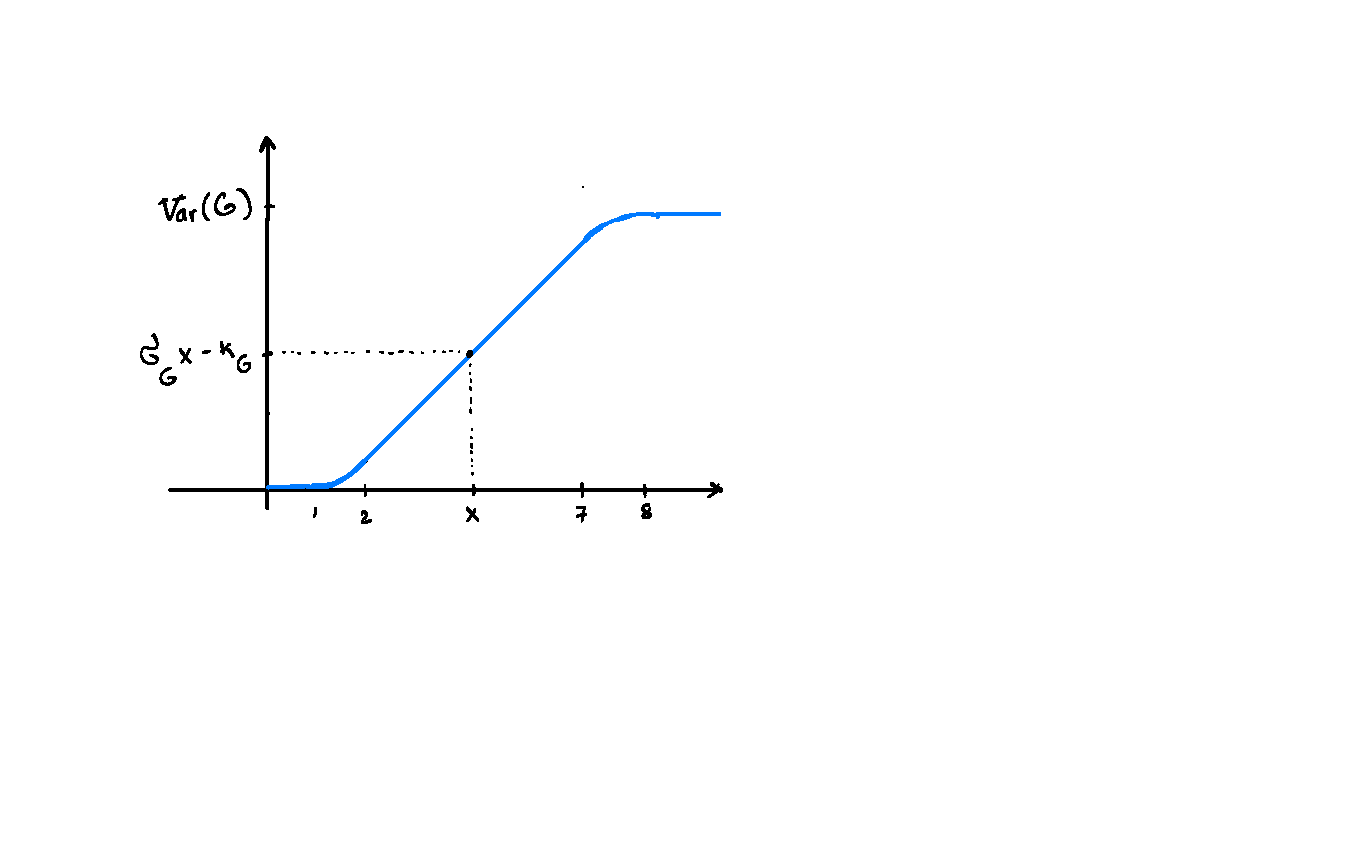
\includegraphics[scale=0.82]{shape_G.pdf}
  \centering
  \caption{The graph of the function $\eta$.} \label{fig:shape_G}
\end{figure}

We notice that $\eta'(x)\leq \frac{3}{2}$, $\forall x\in [0,\infty)$. 
The Hamiltonian diffeomorphism $\Gamma=\phi_{1}^{G}$ generated by $G$
is supported inside $D^{\ast}_{8}(N)$. The Hamiltonian diffeomorphism in the 
statement is the inverse of $\Gamma$:
$$\Psi=\Gamma^{-1}~.~$$

We now describe the Lagrangian $L$. This Lagrangian submanifold is obtained in two steps.
The first is to consider a function $\varphi:N\to [0,\frac{1}{2}]$ as the one constructed in Proposition \ref{prop:Morse} but for $\delta<10$  and define a Lagrangian submanifold $L'$ by
 $$L'=\mathrm{graph}\ (d\varphi)~.~$$
 We denote by $x_{i}$, $1\leq i \leq m$, the critical points of $\varphi$ and take this function $\varphi$ in such a way that $L'\subset \mathrm{Int}(D^{\ast}_{10}(N))$
 and such that $L'\cap D^{\ast}_{9}(N)$ is a disjoint union:
 
 $$L'\cap D^{\ast}_{9}(N) =\coprod_{i=1}^{m} Z_{i}$$ with each
 $Z_{i}\subset W_{i}$ where $W_{i}$ is a small tubular neighbourhoud of $F_{x_{i}}$ (this is the fiber of $T^{\ast}N$ over the critical point $x_{i}$ of $\varphi$). Finally, $L$ is obtained by modifying $L'$ by a Hamiltonian isotopy in such a way that (see  Figure \ref{fig:Lag}):
 $$L\subset \mathrm{Int}(D^{\ast}_{10}(N)) \ , \ L\cap D_{9}^{\ast}(N)=\coprod_{i=1}^{m} F_{x_{i}}\cap D_{9}^{\ast}(N)~.~$$
 \begin{figure}
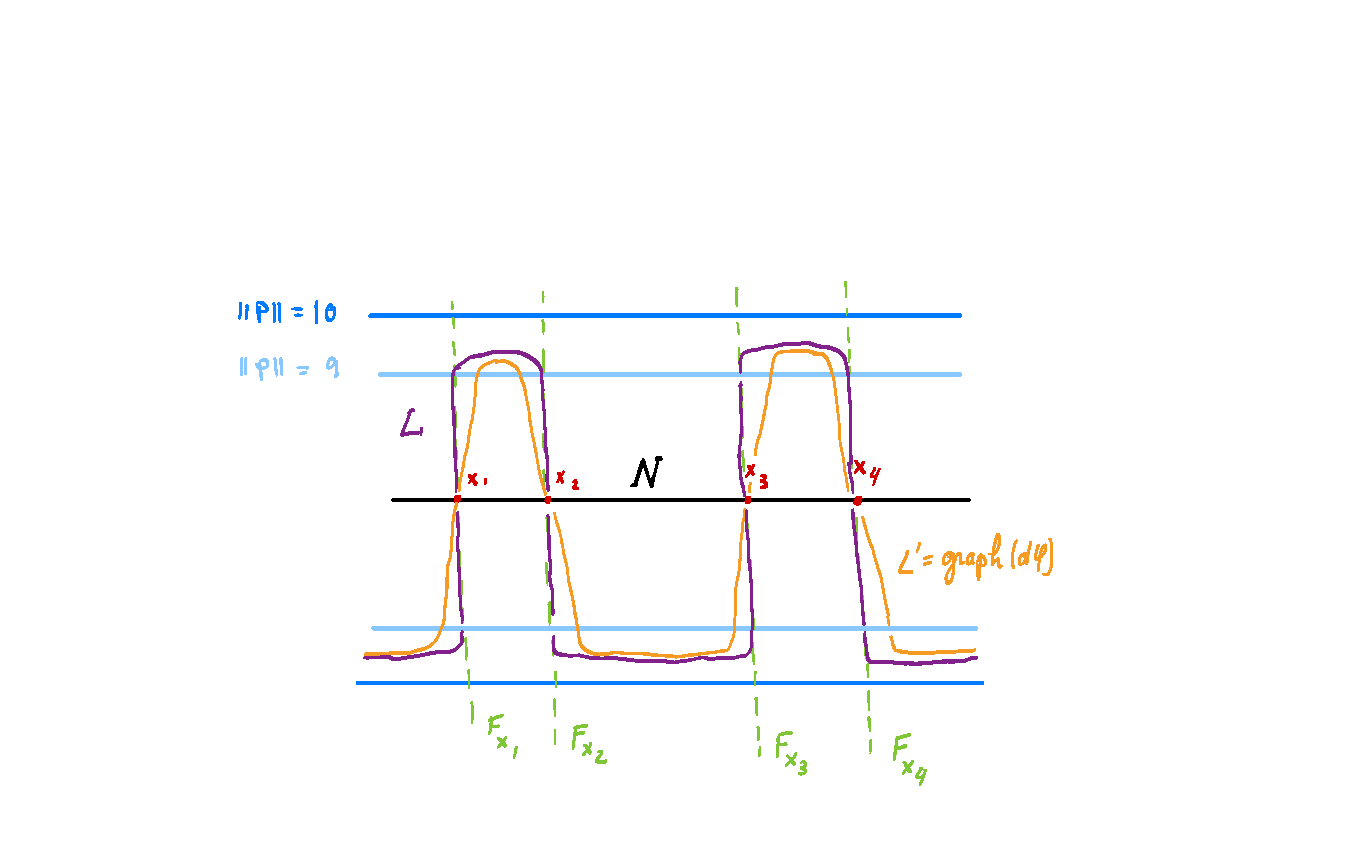
\includegraphics[scale=0.97]{Lag.pdf}
  \centering
  \caption{The shape of the Lagrangian $L$.} \label{fig:Lag}
\end{figure}

 

\begin{rem} The constants $8,9,10$ might need to be replaced by $8 < k < k'$ because in the construction in the proof of Proposition \ref{prop:Morse} we do not directly obtain an upper bound for $||d\varphi||$ while keeping $\mathtt{g}$ fixed (see also Remark \ref{rem:conf_metric}). However, the choice  $k=9$, $k'=10$ is simply a choice of convenience and has no real incidence on the proof. 
 \end{rem}
 
 We will fix some additional notation for the Lagrangian $L$. We let 
 \begin{equation}\label{eq:pieces}
 L_{i}=F_{x_{i}}\cap D^{\ast}_{9}(N)
 \end{equation}
 so that $L\cap D^{\ast}_{9}(N)=\coprod_{i} L_{i}$. We also consider a primitive
 $f_{L}:L\to \R$ of $\lambda|_{L}$ which, up to a shift, is a small perturbation of the primitive $\varphi$ of $\lambda|_{L'}$. In view of this,  we may assume that $f_{L}$ has values inside the interval $[-1,1]$. Of course, $f_{L}$ is constant on each $L_{i}$, with a constant $k_{i}$ on each such component, such that each of these constants belongs to $[-1,1]$ and we may assume
 also that $k_{1}=0$. 
 
 
\subsubsection{Floer homology} In this subsection we establish some properties of certain Floer homology groups that will be essential for the proof. All the Floer homologies considered here are defined in $T^{\ast}(N)$ for an almost complex structure that is convex outside of $D^{\ast}_{8}(N)$.  The maximum principle implies that the Floer trajectories contributing to the relevant differentials are contained in $D^{\ast}_{10}(N)$. The ground field is $\k=\Z_{2}$.

We consider two exact Lagrangian manifolds $K$, $K'$ with primitives
$f_{K}$ and $f_{K'}$, respectively and with fixed choices of gradings, as in the rest of the paper.
In our arguments these Lagrangians $K$, $K'$
are either compact,  included in the interior of  $D^{\ast}_{10}(N)$, or they coincide with fibers $F_{x}$, for $x\in N$. We also consider a Hamiltonian $H: T^{\ast}(N)\to \R$  and an almost complex structure $J=\{J_{t}\}_{0\leq t\leq 1}$ on $T^{\ast}(N)$ that is autonomous and coincides with a convex almost complex structure $J^{\infty}$ 
outside (the interior of) $D^{\ast}_{8}(N)$. We assume that the Hamiltonian $H$ is constant in a neighbourhood of $\partial D^{\ast}_{10}(N)$ and 
that $K$ and $\phi^{-H}_{1}(K')$ intersect transversely. 
We denote by $\mathcal{P}(K,K'; H)$ the Hamiltonian orbits 
$\gamma:[0,1]\to D_{10}^{\ast}(N)$ associated with the Hamiltonian flow $\phi^{H}_{t}$ of $X^{H}$ with $\gamma(0)\in K$, $\gamma(1)\in K'$. There is an action functional on the path-space 
 $$\mathcal{P}(K,K')=\{ \gamma :[0,1]\to D_{10}^{\ast}(N) \ |\ \  \gamma \ \mathrm{smooth,}\  \ \gamma (0)\in K, \ \gamma (1)\in K' \ \}$$
\begin{equation}\label{eq:action1}
\mathcal{A}_{K,K';H}(\gamma)=\int_{0}^{1}H(\gamma(t))dt - \int_{0}^{1}\lambda(\dot{\gamma}(t))dt+f_{K'}(\gamma(1))-f_{K}(\gamma(0))\end{equation}
whose critical points are the elements in $\mathcal{P}(K,K'; H)$. 
As a vector space, the Floer complex $CF(K,K'; H,J)$, when it is defined (thus assuming regularity)
is spanned by $\mathcal{P}(K,K'; H)$.  The differential of the Floer complex counts solutions  $u: \R\times [0,1] \to D_{10}^{\ast}(N)$ of Floer's equation:
\begin{equation}\label{eq:Floer1}
\frac{\partial u}{\partial s} + J_{t} \frac{\partial u}{\partial t} +\nabla_{\rho_{t}} H(u)=0
\end{equation}
where the gradient is taken with respect to the Riemannian metric $\rho_{t}=\omega (- , J_{t})$
and $u(\R\times \{0\})\subset K$, $u(\R\times \{1\})\subset K'$.
We denote by $CF^{a}(K,K'; H,J)$ the subcomplex of $CF(K,K';H,J)$ which is spanned by the Hamiltonian chords $x$ such that $\mathcal{A}_{K,K';H}(x)\leq a$.

 In our application we will have $H=nG$ (with $G$ from (\ref{eq:Ham_G}) )for successively larger values of $n\in \N$. In particular, $H$ is constant outside $D^{\ast}_{8}(N)$.
 This type of Hamiltonian of the form $H=h(||p||)$, with $h$ smooth, has been extensively studied in the literature (see \cite{Bi-Po-Sa:Propagation}\cite{Mac-Sch:top-entr}).  The basic situation of interest for us is when both $K$ and $K'$ are fibers. For convenience, we introduce a special shortened  notation 
$$ C(x,y; n) := CF(F_{x},F_{y}; nG, J)$$
where $F_{x}$ and $F_{y}$ are two different fibers of $T^{\ast}N$.
On both fibers $F_{x}$ and $F_{y}$ we take as primitives the identically zero functions. Regularity can be achieved in this case because, in all our examples, all Floer trajectories will be included inside $D^{\ast}_{8}(N)$ and we have the freedom to pick $\{J_{t}\}$ as desired there while keeping it equal to $J^{\infty}$ outside of $D^{\ast}_{8}(N)$. We emphasize that in the Floer complexes we take into account all the homotopy classes of paths. 
Denote by $$\mathcal{G}_{x,y}=\{\  \bar{\gamma} \ \ |\ \  \bar{\gamma}: [0,\ell]\to N \ \mathrm{is\ a\ geodesic \ } ,\ 
||\dot{\bar{\gamma}}(t)||=1\ \ \ \bar{\gamma}(0)=x, \ \bar{\gamma}(\ell)=y \  \} $$  the geodesic arcs in $N$, parametrized with unit speed length, that go from $x$ to $y$. We denote the length of such a  geodesic arc $\bar{\gamma}$ by $\ell(\bar{\gamma})$. The associated length spectrum is:

$$\mathcal{L}_{x,y}=\{\ \ell(\bar{\gamma}) \ | \ \bar{\gamma}\in \mathcal{G}_{x,y} \} \subset [0,\infty)~.~ $$

Because $(N, \mathtt{g})$ is hyperbolic each homotopy class of paths (with fixed ends) contains a unique geodesic arc in $\mathcal{G}_{x,y}$  and $\mathcal{L}_{x,y}$ is discrete. In particular, $\mathcal{L}_{x,y}$ is countable. It follows, that
the set of quotients $Q\mathcal{L}_{x,y}=\{ \frac{\ell}{n}\ | \  \ell \in \mathcal{L}_{x,y}\ , \  n\in \N^{\ast}\}$ is also countable. We now assume:
\begin{equation}\label{eq:assumption_1}
\sigma_{G}\not \in  Q\mathcal{L}_{x,y}~.~
\end{equation}
This is obviously a generic assumption because the set $Q\mathcal{L}_{x,y}$ is of
zero Lebesgue measure.
\begin{lem}\label{lem:fibers} Under the assumption above the complexes $CF(x,y;n)$ are well defined and, for any $\delta>0$, the number of bars of length $\geq \delta$ in the persistence module $HC(x,y;n)$ increases with $n$ at least as fast as  $\frac{e^{hn}}{hn}$  where $h=\frac{5}{8}h_{top}$ with $h_{top}$ the topological entropy of the geodesic flow.
\end{lem}
\begin{rem}\label{rem:thanks_VG} i. We thank Viktor Ginzburg who suggested to the third author the method to estimate the numbers of bars in $HC(x,y;n)$ as in the proof below.

ii. The quotient $\frac{5}{8}$ in the statement is an artefact of the choice of $\eta$,
it can be brought as close as needed to $1$ by diminishing appropriately the length of the transition regions $(1,2)$ and $(7,8)$ in the definition of $\eta$.
\end{rem}



\begin{proof}  We will use here some of the calculations in \cite{Bi-Po-Sa:Propagation}, see Equation (16) and  Lemma 5.3.2 there, adapted to Lagrangian Floer homology. These calculations imply:
\begin{itemize} 
\item[i.]  The complex $C(x,y;n)$ is well defined and finite dimensional if $n\sigma_{G}\not\in\mathcal{L}_{x,y}$ which is the case due to  (\ref{eq:assumption_1}). The only contributions to the differential of $C(x,y;n)$ is provided by solutions to (\ref{eq:Floer1})
(with $H=nG$) that are contained in $D^{\ast}_{8}(N)$. 
\item[ii.] The generators $\gamma$ of $C(x,y;n)$ are in bijection with geodesic segments $\bar{\gamma}$ in $N$ that join the point $x$ to the point $y$ in the sense that if $\gamma(t)=(q(t),p(t))$, then $q(t)$ is a geodesic from $x$ to $y$ parametrized such that $||\dot{q}(t)||=\ell$; $\bar{\gamma}$ is the same geodesic, re-parametrized with unit speed, and of length $\ell(\bar{\gamma})=\ell$. 
\item[iii.] For each such generator, $\gamma(t)=(q(t),p(t))$, we have that 
$$\frac{p(t)}{r}=\frac{\dot{q}(t)}{||\dot{q}(t)||}\ \ \ \mathrm{with}\ \  r>0\  \ \mathrm{such\ that}\ \ \  n\eta'(r)=\ell~.~$$ In particular, $||p(t)||$ is constant and is equal to $r$ and $\ell\leq n\sigma_{G}$.
\item[iv.] The action of the generator $\gamma$ as above is:
$$\mathcal{A}_{n}(\gamma):=\mathcal{A}_{F_{x},F_{y}; nG}(\gamma)=n\eta(r)- r\ell$$
\end{itemize}
As a result of these remarks, each geodesic arc $\bar{\gamma}$ from $x$ to $y$ 
of length $\ell(\bar{\gamma}) < n\sigma_{G}$ gives rise to a generator of 
$C(x,y;n)$ given by 
\begin{equation}\label{eq:sol}
\gamma(t)=(q(t),\frac{r\dot{q}(t)}{\ell(\bar{\gamma})})
\mathrm{\ \ \ for\ each}\  r\ \mathrm{such\ that\ } \eta'(r)=\frac{\ell(\bar{\gamma})}{n} 
\end{equation}
 where, as above,  $q(t)$ is the geodesic $\bar{\gamma}$ reparametrized such that $||\dot{q}(t)||=\ell(\bar{\gamma})$ (we identify here $T^{\ast}N$ and $TN$ using $\mathtt{g}$).
In view of the properties of the function $\eta$, for a given value $\ell < n\sigma_{G}$, there are exactly two such values $r_{n}(\ell), r'_{n}(\ell)$  with one value, say, $r_{n}(\ell)\in (1,2)$ and the other $r'_{n}(\ell)\in (7,8)$. 

Fix a geodesic arc $\bar{\gamma}$. Denote by $\gamma_{n}$ and $\gamma'_{n}$ the two corresponding Hamiltonian chords associated  to $\bar{\gamma}$ and to the values $r_{n}=r_{n}(\ell(\bar{\gamma}))$ and $r'_{n}=r'_{n}(\ell(\bar{\gamma}))$, respectively, through formula 
(\ref{eq:sol}). They appear as generators of $C(x,y;n)$ as soon as $\sigma_{G}>\frac{\ell(\bar{\gamma})}{n}$, in particular for all $n > \ell (\bar{\gamma})$
(because $\sigma_{G}\geq 1$). 

We now consider the action values of the two relevant generators. We have:
\begin{eqnarray*} \mathcal{A}_{n}(\gamma'_{n})-\mathcal{A}_{n}(\gamma_{n}) =\ n(\eta(r'_{n})-\eta(r_{n})) -\ell(\bar{\gamma}) (r'_{n}-r_{n}) \  \geq \\ \geq  n (\eta(7)-\eta(2)) -7\ell(\bar{\gamma})\geq 5n - 7\ell(\bar{\gamma}) 
\end{eqnarray*} with the last inequality resulting from $\eta(7)-\eta(2)= 5\sigma_{G}$ and $\sigma_{G}\geq 1$. 

Fix $\delta>0$ as in the statement. We deduce: 
\begin{equation}
\label{eq:length_bound} 
\mathcal{A}_{n}(\gamma'_{n})-\mathcal{A}_{n}(\gamma_{n}) \geq \delta \ \ 
\mathrm{if}\ \ 
n\  \geq \  \frac{7}{5} \ \ell(\bar{\gamma})+\frac{\delta}{5} ~.~
\end{equation}
In summary, for $n\geq \ell(\bar{\gamma})$,  $\gamma_{n}$
and $\gamma'_{n}$ appear as generators in $CF(x,y;n)$ and when 
$n\geq \frac{7}{5}\ell(\bar{\gamma})+\frac{\delta}{5}$ their actions are separated by no less than $\delta$.  

The standard Floer homology  $HC^{\infty}(x,y; n)$ vanishes
(forgetting the persistence structure is indicated by the superscript $\infty$) and the Floer differential in $C(x,y; n)$ is very simple.
Indeed, Floer trajectories can only join Hamiltonian chords that project to  paths in $N$ in the same homotopy class. Given that each geodesic in $\mathcal{G}_{x,y}$
is unique in its homotopy class, it follows that when $n>\frac{7}{5}\ell(\bar{\gamma})+\frac{\delta}{5}$, we have $d(\gamma'_{n})=\gamma_{n}$ (recall that we work over $\Z_{2}$ and that $HC^{\infty}(x,y;n)$ vanishes) and the 
couple $(\gamma_{n},\gamma'_{n})$ defines a bar of length at least $\delta$ in the
persistence module $HC(x,y;n)$. Thus, for $n$ big enough, the number of bars of length at least $\delta$ in $HC(x,y;n)$ is at least the number of geodesic arcs in $\mathcal{G}_{x,y}$ of length $\leq \frac{5}{8}n < \frac{5}{7} n(1 -\frac{\delta}{5n})$.
By classical results, such as in %\cite{Buser},
 \cite{Parry_Pollicott:Zeta} Chapter 9, 
the number of geodesics in $\mathcal{G}_{x,y}$ of length less than $T$ increases
as fast as $$\frac{e^{Th_{top}}}{Th_{top}}~.~$$ By replacing $T$ with $\frac{5}{8} n$
we obtain the result.
 \end{proof}

We next turn our attention to the filtered complex  
 $$C(x ,L; n):=CF(F_{x}, L; nG,J)$$
 where $L$
is the Lagrangian fixed in \S\ref{subsubsec:choices}.  Recall that $L$ has the property $L\cap D^{\ast}_{9}(N) =\cup_{i} L_{i}$ with $L_{i}=F_{x_{i}}\cap D^{\ast}_{9}(N)$ (see (\ref{eq:pieces})).
 
We assume that $x\not= x_{i}$ for all the critical points $x_{i}$ of $\varphi$ and we add two additional assumptions relative to $F_{x}$,$L$, and $G$:
\begin{equation}\label{eq:sigma_2}
\sigma_{G}\not\in Q\mathcal{L}_{x,x_{i}}, \ \ \forall x_{i} \end{equation}
As mentioned after (\ref{eq:assumption_1}), this is a generic assumption on the choice
of $\sigma_{G}$. Note that:
\begin{equation}\label{eq:inters}
L\cap F_{x}= \{z_{x}\} \subset D^{\ast}_{10}(N)\backslash D^{\ast}_{9}(N)~.~
\end{equation}
To make sense of this recall from \S\ref{subsubsec:choices} that $L$ is a small deformation of $L'$ which is the graph of $d\varphi$. It follows that, under the assumption that $x\not= x_{i}$, $\forall i$, we have that $F_{x}$ intersects $L$ in a single point - denoted by $z_{x}$ - which lies outside of $D^{\ast}_{9}(N)$. 
 
Given that $G$ is constant outside of $D^{\ast}_{8}(N)$ we deduce that the  underlying
 vector space of $C(x,L; n)$ can be written as:
 \begin{equation} C(x,L;n)=\oplus_{i}\Sigma^{k_{i}} C(x,x_{i};n)\oplus \Z_2 \langle z_{x} \rangle ~.~
 \end{equation} 
 Moreover, for the same reason, the complexes $C(x,x_{i},n)$ are finite dimensional over $\Z_{2}$. The shift $\Sigma^{k_{i}}$ appears here because the value of the primitive 
 $f_{L}$ on the component $L_{i}$ is not $0$, but rather $k_{i}\in [-1,1]$. The action of the point $z_{x}$ is $f_{L}(z_{x})$, see (\ref{eq:action1}). Denote by $d^{x_{i};n}$ the differential of the complex $C(x,x_{i};n)$ and let 
 $D^{n}$ be the differential of the complex $C(x,L;n)$.  Finally, recall that for a filtered chain complex $C$ we denote by $C^{a}$ the filtration $\leq a$ subcomplex. 
 \begin{lem} \label{lem:defor}With the notation above there exists a constant $\xi>0$ that depends
 on $(N,\mathtt{g})$, on $L$, on $x$, and on the almost complex structure $J$ (but not on $n$) such 
 that $$ D^{n} = \oplus_{i} d^{x_{i};n} + \bar{D}^{n}$$ with the property that
 $$\bar{D}^{n}(C^{\alpha}(x,L;n))\ \subset \ C^{\alpha-\xi}(x,L;n) \ , \ \forall \ \alpha  
 ~.~$$
 \end{lem}
 
 \begin{proof} The Floer strips that contribute to the differential $D^{n}$ are of two types: 
 those that stay inside $D^{\ast}_{8}(N)$ - in this case they appear in one of the differentials
 $d^{x_{i};n}$, and strips $u$, called below of {\em second type}, such that $\mathrm{Im}(u)\not\subset D^{\ast}_{8}(N)$. Recall that the Lagrangian $L$ coincides with a union of fibers
 inside $D^{\ast}_{9}(N)$. Using the maximum principle,  this implies that 
 any strip $u$ of the second  type has to reach the non-fiber-like region of $L$. In other words, there exists a point $(s_{0},0)\in \R\times\{0\}$ such that $u(s_{0},0)\not\in D^{\ast}_{9}(N)$. 
 The aim of the proof is to show that there is a constant $\delta$, as in the statement, such 
 that the energy
 $$E(u)=\int ||\frac{\partial u}{\partial s}||^{2}\ dsdt $$
 satisfies $E(u)\geq \delta$ for any strip $u$ of the second type.
 
The argument is based on standard monotonicity  results such as in Sikorav \cite{Sik:est}. 
The first step is to fix the constant $\xi$. Let $K= D^{\ast}_{9}N\backslash \mathrm{Int}(D^{\ast}_{8.5}(N))$. The results in  \cite{Sik:est} - see Proposition 4.7.2 there -  imply that there exist positive constants $r_{0}$ and $C$ that depend only on $J$, $(N,\mathtt{g})$, and $L$ with the following property.
For each point $p\in L\cap K$, if $v:\Sigma\to K$  is a
$J$-holomorphic curve with $\Sigma$ compact with boundary, such that:
\begin{itemize}
\item[i.] There is  some point $x\in \partial\Sigma$ with $v(x)=p$,
\item[ii.] $v(\Sigma)\subset B_{r}(p)\subset K$ with $r\leq r_{0}$ (where $B_{r}(a)$ is the ball in $T^{\ast}(N)$ of radius $r$ with center $a$),
\item[iii.] $v(\partial \Sigma)\subset \partial B_{r}(p)\cup L$,
\end{itemize}  
 then the symplectic area $A(v)$ of $v$ satisfies:
 $$A(v)\geq Cr^{2}~.~$$
 
Now pick some $r'<r_{0}$ such that for each point in $z\in L\cap (D^{\ast}_{8.8}(N)\backslash \mathrm{Int}(D^{\ast}_{8.6}(N)))$ we have 
\begin{equation}\label{eq:dep_x}
B_{r'}(z)\subset K\backslash F_{x}.
\end{equation}
 We put:
 $$\xi= C(r')^{2}/2~.~$$
 

 With this notation we return to a Floer strip of the second type $u:\R\times [0,1]\to D^{\ast}_{10}(N)$. We want to show  $E(u)\geq \xi$. We know that there is some $s_{0}$ with the property that the point $u(s_{0},0)$ is in $L\backslash D^{\ast}_{9}(N)$. Moreover, at least one of the asymptotic limits of $u$ is a Hamiltonian chord of $nG$ (for some $n$) and is therefore inside $D^{\ast}_{8}(N)$. It follows that there is also  some point
 $s_{1}\in \R$ such that $p=u(s_{1},0)\in  L\cap (D^{\ast}_{8.8}(N)\backslash \mathrm{Int}(D^{\ast}_{8.6}(N)))$.
 
 
 Denote by $u_{r}$ the restriction of $u$ to the set $S_{r}=u^{-1}(B_{r}(p))\subset \R\times [0,1]$ for $ 0 < r \leq r'$. By making use of Sard's theorem, for a generic choice of $r$ the set $S_{r}$ is a compact surface with boundary. We pick such a regular $r_{1}> \frac{r'}{\sqrt{2}}$. We notice that $u_{1}:S_{r_{1}}\to B_{1}(p)$ has the property that $u_{1}(\partial S_{r_{1}})\subset \partial B_{r_{1}}(p)\cup L$. We also have, of course, $u_{1}(S_{r_{1}})\subset B_{r_{1}}(p)\subset K$. Recall that $G$ is constant outside of $D^{\ast}_{8}(N)$ and thus $\nabla (nG)$ vanishes on $K$.
 As a result $u_{1}$ is $J$-holomorphic and thus we obtain:
 $$E(u)\geq A(u_{1})\geq Cr_{1}^{2}\geq \xi$$
 which concludes the proof. 
   \end{proof}
  
  \begin{rem}\label{rem:dep_onx}
  The constant $\xi$ in the lemma depends very lightly on the point $x$. Indeed, if we  assume that $F_{x}$ does not intersect a fixed neighbourhood
 $U$ of $L\cap D^{\ast}_{9}(N)$, then we may replace condition
 (\ref{eq:dep_x}) by $B_{r'}(z) \subset K\cap U$ and under this assumption
 $\xi$ is independent of $x$ and only depends on $L$, $J$, $(N,\mathtt{g})$, and $U$.
  
  \end{rem}
  
  
  
  \subsubsection{An auxiliary algebraic  result}
We will next use the following simple  statement. 
  
  \begin{lem}\label{lem:bar_counts2}
  Suppose that $C$ is a filtered, finite dimensional chain complex over $\Z_2$ that is $\Z_2$-graded. 
  Fix $\delta>0$.
  If the differential $D$ of $C$ can be written as
  $$D=d+D'$$ with $d^{2}=0$ and $D'$ such that $D'(C^{\alpha})\subset C^{\alpha-\delta}$
  for all $\alpha\in\R$, then for any $\epsilon<\delta$, we 
  have $$\#(\ \mathcal{B}^{\epsilon}_{H(C))}\ )\geq \#(\ \mathcal{B}^{\epsilon}_{H(C,d)} \ )~.~$$
  \end{lem}
  
  \begin{proof}
  The result is most likely known by experts but we give a proof for completeness. We denote by 
  $C_{0}$ the complex $(C,d)$. It is easy to see that it is enough to show the statement when $C_{0}$ is acyclic which we will now assume. We write 
  $C_{0}$ as a direct sum of terms $E_{2}(a,b)$   with filtrations given by a valuation $v$ with values in $\R$ (see \S\ref{subsec:pers}). There are two types of terms of this form,
  those such that $v(a)\leq v(b)\leq v(a)+\epsilon$ - they will be denoted
  by $E_{2}^{s}(a,b)$, and those with $v(b)> v(a)+\epsilon$, denoted by 
  $E_{2}^{l}(a,b)$. The number  $n_{l}$ of terms of type $E_{2}^{l}$ equals the number of bars in $\mathcal{B}_{HC_{0}}$ of length greater than $\epsilon$. We now consider one $E_{2}^{s}$ term, $E_{2}^{s}(a_{0},b_{0})$,
such that $v(b_{0})-v(a_{0})\leq \epsilon$ is minimal among all terms $E_{2}^{s}$. We let $C_{1}$ be the subspace of $C$ generated by the generators of $C$ different from $\{a_{0},b_{0}\}$ so that as $d$-chain complexes we have
$C_{0}=E^{s}_{2}(a_{0},b_{0})\oplus C_{1}$.    We consider
the element $$a'_{0}= a_{0} + D'(b_{0})~.~$$ It has the property $a'_{0}=D(b_{0})$. We notice that $v(a'_{0})=v(a_{0})$ because $\epsilon < \delta$ and thus $v(D'(b_{0})) < v(a_{0})$. Therefore, we also have $D'(b_{0})\in C_{1}$.
Let $$ E_{2}(a'_{0}, b_{0})=\Z_2 \langle \  a'_{0},\  b_{0} \ : \ D(b_{0})= a'_{0}, D(a'_{0})=0 \ \rangle ~.~$$ 
Then $E_{2}(a'_{0}, b_{0})$ is a $D$-subcomplex of $C$. We have the projection $p_{1}: C\to C_{1}$ defined on generators as the identity on $C_{1}$ and that sends $b_{0}$ to $0$, and $a_{0}$ to $D'(b_{0})$. This projection has as kernel $E_{2}(a'_{0}, b_{0})$  and is 
filtration preserving in the sense that it sends $C^{\alpha}$ to $C^{\alpha}_{1}$, for all $\alpha\in\R$.
The differential $D$ induces a differential $D_{1}$ on $C_{1}$ which is the unique linear map making  $p_{1}$ a chain map. Moreover, $D_{1}$ can be written:
$$D_{1}= d + D'_{1}$$
where $D'_{1}=p_{1} \circ D'$. It is easy to see that $D'_{1}$ also drops the filtration by
at least $\delta$, just as $D'$ in the statement. Assume for the moment that the map $p_{1}$ admits a section $j_{1}: (C_{1}, D_{1}) \to (C, D)$ which is a filtration preserving chain map. In that case, we can reapply iteratively the same procedure to $(C_{1},D_{1})$
to successively eliminate all the $E_{2}^{s}(a,b)$'s. We are left at the end with a complex $(C_{k}, D_{k})$ whose dimension is $2 n_{l}$  and whose differential $D_{k}=d+D'_{k}$ drops filtration by more than $\epsilon$ ($d$ drops differential by more than $\epsilon$ on $C_{k}$, and $D'_{k}$ by at least  $\delta > \epsilon$). As a result, all the bars 
in $HC_{k}$ are longer than $\epsilon$ and there are at least $n_{l}$ of them.
By our iterative construction, $(C_{k},D_{k})$ is a filtration preserving retract of $(C,D)$ and therefore the number of bars of length more than $\epsilon$ in $HC$ is at least $n_{l}$, as claimed. 

Thus, to finish the proof we are left to construct the section $j_{1}$. 
We will construct a linear map $j_{1}:C_{1}\to C$ that is filtered and has the property that $p_{1}\circ j_{1}=id$ and, additionally, $\mathrm{Im}(j_{1})$ is
a subcomplex of $C$. This implies that $j_{1}$ is also a chain map.
As a vector space, we have the splitting  $C=E_{2}(a_{0}',b_{0})\oplus C_{1}$.
Let $x\in C_{1}$. There are two possibilities. Assume that, relative to this splitting, $D(x)=w\in C_{1}$. In that case, we put $j_{1}(x)=x$. On the other hand, assume that $D(x)= a_{0}'+w$ with $w\in C_{1}$. In this case we put  $j_{1}(x)= x+ b_{0}$. We notice $v(x)\geq v(b_{0})$. Moreover, $D(x+b_{0})\in C_{1}$ and, with this definition, $j_{1}$ is different from the identity only in degree $|a_{0}|+1$.  We also have that $j_{1}$ is filtration preserving in the stronger sense that $v(j_{1}(y))=v(y)$ for all $y\in C_{1}$. It is clear that $p_{1}\circ j_{1}=id$.  We now want to remark that $\bar{C}_{1}=\mathrm{Im}(j_{1})$ is closed with respect to $D$. First, the construction
above means that for each $x\in \bar{C}_{1}$,  $D(x)$ can not 
have the form $a'_{0}+w$, $w\in \bar{C}_{1}$. Indeed,  all $x\in \bar{C}_{1}$ in degree $|a_{0}|+1$ satisfy $D(x)\in C_{1}$ and $C_{1}$ and $\bar{C}_{1}$ coincide in degree $|a_{0}|$. Now assume that for some $x\in \bar{C}_{1}$, $D(x)=b_{0} + \zeta$, $\zeta\in \bar{C}_{1}$.  Then  $0=D^{2}(x)= a'_{0} + D(\zeta)$ which leads to a contradiction. Thus $\bar{C}_{1}$ is a $D$-subcomplex in $C$ and this concludes the proof.
 \end{proof}
 
 \begin{rem} We have used at certain points in the proof the fact that we work over $\Z_2$ but the result remains true with a similar proof over any field $\k$.
 
 \end{rem}
 
\subsubsection{The main step in the proof of Proposition \ref{cor:hyp_ent}} The aim of this subsection is to  show:

\begin{lem}\label{lem:parrila}  For $\epsilon$ sufficiently small and for  any $\epsilon$-approximating family $\mathcal{F}_{\epsilon}$ for $\lag^{(ex)}(D^{\ast}_{10}N)$ in $\msc_{p}(10)$, with $\nu(p)$ sufficiently small - as in Theorem \ref{thm:nearby}, thus with $\F_{\epsilon}$ consisting of fibers - there is a Hamiltonian isotopy $\Psi$ with support in $D^{\ast}_{10}(N)$, a Lagrangian $L$, both as in \S \ref{subsubsec:choices}, and one fiber, $F_{x}\in \F_{\epsilon}$ such that the number of bars:
$$\# (\mathcal{B}^{\epsilon}_{HF(F_{x},\Psi^{n}L)})$$ grows in $n$ at least as fast as  $\frac{e^{hn}}{hn}$, where $h$ is the constant in Lemma \ref{lem:fibers}. 
\end{lem}

%Notice that we use here the  local $\epsilon$-approximating data $(\Phi,\F_{\epsilon})$, %as in \S\ref{subsubsec:local_approx_d} and in Theorem \ref{thm:nearby}, and not the %ambient data $(\Phi',\F'_{\epsilon})$ in the statement of Proposition \ref{cor:hyp_ent}.
%
\begin{proof}
We start the argument by choosing a Lagrangian $L$ as in \S\ref{subsubsec:choices}.  We also fix a small neighbourhood $U$ of $L\cap D_{9}^{\ast}(N)$. We pick $\delta$ to be the constant given by Lemma \ref{lem:defor} under the assumption that $F_{x}\cap U=\emptyset$.
As noted in Remark \ref{rem:dep_onx} this constant is then independent 
of $x$. We pick $\epsilon < \delta$ and let $\F_{\epsilon}$ be an $\epsilon$-approximating family for $\msc_{p}(10)$. If $\epsilon$ is small enough there is 
at least one element $F_{x}$ of $\F_{\epsilon}$ that does not intersect $U$ (this follows from the fact that when $\epsilon\to 0$ the union $\cup_{F\in \F_{\epsilon}}F$ becomes dense in $D^{\ast}_{10}(N)$).
At this point we can pick the Hamiltonian $G$. We pick $G$ as in \S\ref{subsubsec:choices} subject to the assumption (\ref{eq:sigma_2}) which is generic.  This means that the complex $CF(F_{x}, L; nG, J)$ is defined for 
each $n$, it is finite dimensional over $\Z_{2}$, and that it satisfies the statement 
in Lemma \ref{lem:defor}.
This means that 
$$CF(F_{x},L;nG,J)=\oplus \Sigma^{k_{i}}CF(F_{x},F_{x_{i}};nG,J)\oplus \Z_2 \langle z_{x}\rangle $$
as filtered vector spaces, with $F_{x_{i}}$ as in (\ref{eq:pieces}) and 
that the differential $D^{n}$ of $CF(F_{x},L;nG,J)$ satisfies:
$$D^{n}=\oplus_{i}d^{x_{i};n}+\bar{D}^{n}$$ with 
$\bar{D}^{n}$ dropping filtration by at least $\xi$ and with $d^{x_{i};n}$ the differential in $CF(F_{x},F_{x_{i}};nG,J)$. 
In this situation we can  apply Lemma \ref{lem:bar_counts2}
to deduce :

$$\# (\mathcal{B}^{\epsilon}_{HF(F_{x},L;nG,J) })\geq  \sum_{i}\# (\mathcal{B}^{\epsilon}_{HF(F_{x},F_{x_{i}};nG,J)})~.~$$
We use  Lemma \ref{lem:fibers} to conclude that
$\# (\mathcal{B}^{\epsilon}_{HF(F_{x},L;nG,J) })$ increases in $n$ as fast 
as $\frac{e^{hn}}{nh}$.

The argument concludes by noting that by the naturality of Floer's equation, there is a filtered chain isomorphism:
$$CF(F_{x}, \Psi^{n} L; 0, J_{n})\to CF(F_{x},L;nG, J)~.~$$ 
Here $\Psi = \Theta^{-1}$ where $\Theta=\phi_{1}^{G}$ is induced by the Hamiltonian flow of $G$. The almost complex structure
$J_{n}$ is such that $\Theta^{n}_{\ast}J_{n}=J$. Because $G$ is constant outside 
$D^{\ast}_{8}(N)$, the almost complex structures $J_{n}$ coincide with $J$ there and thus the complexes $CF(F_{x}, \Psi^{n} L; 0, J_{n})$ are well defined
because $|| - ||^{2}$  is  $J_{n}$- convex outside $D^{\ast}_{8}(N)$. The persistence
module $HF(F_{x}, \Psi^{n} L; 0, J^{*})$ is in fact independent of the almost complex structure $J^{\ast}$, as long as it coincides with $J$ outside $D^{\ast}_{8}(N)$.

\end{proof}

\subsubsection{End of the proof of Proposition \ref{cor:hyp_ent}}\label{subsubsec:back_to_E} 
The constructions in the subsections above can be appropriately rescaled so  that they take place 
in the unit disk bundle $D^{\ast}N$ instead of $D^{\ast}_{10}(N)$ and, further, 
this disk bundle is included in the total space of  the Lefschetz  fibration $\bar{h}:E\to \mathbb{C}$ that was instrumental in the proof of Theorem \ref{thm:nearby}.
 Moreover, we may assume as in \S\ref{subsec:exact-seq} that the TPC $\epsilon$-approximating
 family $\F'_{\epsilon}$ consists of Lagrangian spheres $\hat{S}_{x_{i}}$ that each intersects 
 $D^{\ast}N$ in a fiber $F_{x_{i}}$ of $D^{\ast}N$. The collection of these fibers is precisely 
 the $\epsilon$-TPC-approximating family $\F_{\epsilon}$, see \S\ref{subsubsec:complex_Lag} for a brief
 recap of the context.
 
 \
 
We now recall the conclusion of  Lemma \ref{lem:parrila}: the number of bars $\# (\mathcal{B}^{\epsilon}_{HF(F_{x},\Psi^{n}L)})$ grows in $n$ at least as fast as  $\frac{e^{hn}}{hn}$. It is easy to see that the constructions leading to this result (that all take place in $D^{\ast}(N)$) can be adjusted so  that we have the same rate of growth for  $\# (\mathcal{B}^{4\epsilon}_{HF(F_{x},\Psi^{n}L)})$ which is what we will assume from now on.
Recall that $F_{x}$ is one of the fibers in the approximating family $\F_{\epsilon}$ and $\Psi^{n}L\subset  \mathrm{Int}(D^{\ast}N)$. 
Therefore, $F_{x}\cap \Psi^{n}L= \hat{S}_{x}\cap \Psi^{n}L \subset \mathrm{Int}(D^{\ast}N)$.  Due to the convexity of $\partial D^{\ast}N$ we deduce that the Floer complexes $CF(F_{x}, \Psi^{n}L;0, J_{n})$ and $CF(\hat{S_{x}}, \Psi^{n}L;0,J_{n})$ coincide. 
As a result 
$$\# (\mathcal{B}^{4\epsilon}_{HF(\hat{S}_{x},\Psi^{n}L)})$$  also grows in $n$ at least 
as fast as  $\frac{e^{hn}}{hn}$.

Both $\hat{S}_{x}$ and $\Psi^{n}L$ are Yoneda modules so that
$HF(\hat{S}_{x},\Psi^{n}L)=\hom_{\mathscr{D}_{p}(E)}(\hat{S}_{x},\Psi^{n}L)$. 
As a result $\hbar  (\Psi; L, \hat{S_{x}}, 4\epsilon)$, as defined in  (\ref{eq:bar-code_ent}) does not vanish. Given that $G_{\F'_{\epsilon}}=\oplus_{S\in \F'_{\epsilon}}S$
we also have $\hbar (\Psi; L, G_{\F'_{\epsilon}},4\epsilon)>0$.
At this point we can apply Corollary \ref{cor:ineq_bar2}
 and we deduce 
 $$ h^{r}_{\Phi',\F'_{\epsilon}}(\Psi; L,2\epsilon)>0$$
 which is the desired statement. \qed
 
% !TEX root = approx8.tex


\subsection{Complexity of equators on $S{^2}$}\label{subsec:tb_S2}
The aim of this subsection is to complete the proof of Corollary \ref{cor:no-t-b} by showing that the space of equators on $S^{2}$
endowed with the spectral metric is not totally bounded.  We will use the notation in \S\ref{sec:split-app}. In particular,
the set of equators on the $2$-sphere is denoted by
$\lag^{\text{(mon,} \mathbf{0} \text{)}}(S^2)$. Here 
the notation reflects the fact that equators are monotone, and $\mathbf{0}$ indicates that the $\Z_{2}$-number of Maslov -$2$  $J$-holomorphic disks with boundaries on an equator $L$, and passing through a fixed point $x\in L$, vanishes. Recall  from Proposition \ref{OCS2} that this class of Lagrangians
is retract approximable  with an $\frac{1}{4N}+2\nu(p)$-approximating family of the form
$L_{1},\ldots, L_{N}$ where $L_{i}$ is a great circle passing through the north and south poles of $S^{2}$ and is  at angle $\frac{\pi}{2N}$ from $L_{i-1}$. We fix  $L_{1}$ such that it passes through  the point $(1,0,0)$. We assume that the metric
on $S^{2}$ is such that its area is equal to $1$.

%\ocnote{Need to add a Remark in Section 4, after the Proposition \ref{OCS2} to note that the result implies approximability of the respective class of Lagrangians with {\em the spectral metric}; same thing for the torus}.

Notice that in this case, by contrast to the case of $M=D^{\ast}N$, the approximating data $(\Phi, \F)$ is simpler in the sense
that the categories $\mathscr{Y}_{\epsilon,\eta}$ do not depend
on $\epsilon$, the only dependence is on $p$ (we may assume $\eta=\nu(p)$) and for each $N$, the family $\mathcal{E}(N)=\{L_{1},\ldots, L_{N}\}\subset \mathcal{E}$ where $\mathcal{E}$ is the set of all great circles passing through the two poles.   
\begin{prop} \label{prop:complex_S2}
There exists a Hamiltonian diffeomorphism $\Psi\colon S^{2}\to S^{2}$,  $L\in\mathcal{E}$,   $N\in \N$, and  $\epsilon' \geq  2 (\frac{1}{4N}+2\nu(p))$, such that:
\begin{equation*}
N^{r}(\Psi ^{k}L, \mathcal{E}(N), \epsilon') \stackrel{k\to \infty}{\longrightarrow} \infty~.~
\end{equation*}
\end{prop}
In view of this proposition and of Remark \ref{rem:tb_complex} it follows that the space
$(\lag^{\text{(mon,} \mathbf{0} \text{)}}(S^2), d_{\gamma})$
is not totally bounded.

\begin{proof}[Proof of Proposition \ref{prop:complex_S2}]
We start by identifying $\Psi$: this is the Dehn twist along the 
horizontal equator on the sphere with support inside the annulus
$$U=\{(x,y,z)\in S^{2} \ |  -a  < z < a  \}$$ with $a>0$ picked in such
a way that the area of $U$ is smaller than $\frac{1}{4}$.
Next we pick $L$ to be the great circle on $S^{2}$ that passes through the north and south poles and also through the 
point $(0,1,0)$. Note that $L$ intersects transversely $L_{1}$, the first element in the family $\mathcal{E}(N)$.

The idea of the proof is simple: we would like to use an analogue of the first  inequality in Corollary \ref{cor:ineq_bar2}, for a fixed $\epsilon'$ and some $N$ (with $\mathcal{E}(N)$ in the place of $\F'_{\epsilon}$),  and then show that the number of bars of length larger than $2\epsilon'$ in 
$HF(L_{1},\Psi^{k}L)$ goes  to infinity with $k$. The key issue to be resolved is that we work here in the monotone context and over the Novikov field $\La$, as in \S\ref{sb:fuk-mon}. As a result, the algebraic
results in Proposition \ref{prop:lower-bd}  and (\ref{eq:ineq-r-bar}) need to be adjusted to this context. This can be achieved by using the results of Usher-Zhang \cite{Usher-Zhang:perh} as we will briefly
review next.

Assume that $C$ is a finite dimensional, filtered chain-complex defined over the Novikov field  $\La$.  The homology $H(C)$ is a persistence module in the classical sense over the field $\Z_{2}$.  However, counting bars in the usual way does not make sense because if one bar of type $[a,b)$ appears, all translates of type $T^{\alpha}[a,b)$ also appear for all $\alpha\in\R$.  The tools required to deal with this problem are introduced in \cite{Usher-Zhang:perh} together with a specific terminology.  First, the methods in 
\cite{Usher-Zhang:perh} apply to rings of Novikov type but more general than our choice here, that are denoted there by $\La^{\mathcal{K},\Gamma}$ where $\mathcal{K}$ is the ground field ( $\Z_{2}$ in our case), and $\Gamma$ is an additive subgroup of $\R$. In our case, $\Gamma=\R$. Moreover, \cite{Usher-Zhang:perh} applies to so-called {\em non-Archimedean normed vector spaces that are orthogonalizable} which means vector spaces $C$ over $\La$ endowed with a filtration function $\ell :C\to \R\cup \{-\infty\}$ with the properties typical for action functionals together with a property of admitting special ``orthogonal'' bases. Such complexes are called of Floer-type  in  Definition 4.1 in \cite{Usher-Zhang:perh} and, in particular, all Floer complexes in our paper fit into this class.  All Floer-type complexes   will always be finite dimensional over $\La$ in our case. To such a Floer-type chain complex $C$ \cite{Usher-Zhang:perh} assigns
a bar-code $\bar{\mathcal{B}}_{HC}$, called there the {\em concise} bar-code of $C$, that consists
of intervals of non-negative length, possibly infinite and that all have $0$ as
lower bound (this is, of course, different from the case considered earlier in this section; the fact that the lower bound of the bars is always $0$ reflects  the issue mentioned above having to do with the action of $\La$). It is shown that such a bar-code determines $C$ up to filtered chain-homotopy equivalence (which explains why we use $H(C)$ in the notation). The construction of this barcode parallels the standard construction over a non filtered field: it goes through a writing of the differential of the complex $C$, $d:C\to C$,
 in  a special basis over $\La$ such that the matrix of the differential is upper triangular and only contains $0$'s and $1$'s, with at most a single $1$ on each row and column.  We denote by $\bar{\mathcal{B}}^{\delta}_{H(C)}$ the 
barcode formed by eliminating from $\bar{\mathcal{B}}_{H(C)}$ all
the bars of length $\leq\delta$, just as in  \S\ref{subsec:pers}. The construction of the barcode $\bar{\mathcal{B}}_{H(C)}$ easily shows that the analogue of 
Lemma \ref{lem:noc-chains} remains true in this context with the place of 
$V$ being taken by a Floer-type finite dimensional complex over $\La$ and 
with $\bar{\mathcal{B}}$ in the place of $\mathcal{B}$. As result 
 Proposition \ref{prop:lower-bd}  and (\ref{eq:ineq-r-bar}) remain also true
 with the  modification that the base $A_{\infty}$-category is a Fukaya
 filtered category  over $\La$ and that $\bar{\mathcal{B}}$ takes the place of $\mathcal{B}$. 
 
 In brief, to prove the proposition we need to show that 
 \begin{equation}\label{eq:estimate_bars3}
 \#\  \left(\bar{\mathcal{B}}^{2\epsilon'}_{HF(L_{1},\Psi^{k}L)}\right)\stackrel{k\to\infty}{\longrightarrow} \infty ~.~
 \end{equation} 

At this point we pick the value  $\epsilon'= \frac{1}{32}$. We will consider the complex $CF(L_{1}, \Psi^{k}L)$ defined over $\La$. The generators of this complex  are the intersection points $L_{1}\cap \Psi^{k}L$. The number of these intersection points is $2k+2$: two of them
are the north and south poles and there are two others for each successive application of $\Psi$.  Floer trajectories are holomorphic and by using the open mapping theorem it is easy to see that if a Floer trajectory starts at a point $\in L_{1}\cap \Psi^{k}L \cap U$ then it  can not remain entirely inside $U$ and thus it fills a connected region of $S^{2}\backslash ( U \cup L_{1} \cup L)$. As a result each such Floer trajectory has area at least $\frac{3}{32}$. At the same time the Floer homology with $\Z_{2}$ coefficients $HF(L_{1}, \Psi^{k}L;\Z_{2})$ is well defined (this is obtained by making $T=1$) and is isomorphic
to $HF(L_{1}, L;\Z_{2})$ which is of dimension $2$ over $\Z_{2}$ and is generated by the north and the south poles. It follows that $\bar{\mathcal{B}}_{HF(L_{1},\Psi^{k}L)}$ contains at least $k$ bars and each of them is of length more than $\frac{2}{32}=2\epsilon'$. This concludes the proof.
\end{proof}


\begin{rem} \label{rem:equators1}
It is easy to reformulate Proposition \ref{prop:complex_S2} in terms of the non-vanishing of an entropy type measurement that one may call $\epsilon$-weighted  {\em slow} (categorical) entropy which is defined just as in formula (\ref{eq:cat_entropy2}) except that $\log (n)$ is used at the denominator, in the place of $n$. In these terms, what we have shown in the proof above is that the slow $\epsilon$-weighted retract entropy of $\Psi$ with respect to $L$, both chosen as in the proof, is  at least $1$ as soon as $\epsilon \leq \frac{1}{32}$. Because  $\Psi$ is a Hamiltonian diffeomorphism, it is easy to see that for $\epsilon=\infty$ the slow entropy vanishes. Relations between entropy and Floer theoretic calculations have been initiated in  \cite{FS:vol-growth}. See  \cite{DawFlBar} \cite{DawA3} for some other results involving bar-code entropy estimates.





\end{rem}

 